\chapter{Results}
In this chapter, we will show the results obtained from several tests using hierarchical clustering over Decidim Barcelona proposals data.

First, we describe Decidim Barcelona proposals to understand the challenge and limitation for clustering this data. Then, we present two sets of results: a positive result using proposals from very different categories and a different ground truth, and a negative result using proposals from one category. We decided to start with a controlled set of clearly different proposals. Then, we carried the same experiments over a set of proposals from one category that could represent the whole dataset more properly.

\section{Dataset Details}
In our experiments, we used proposals represented by their title and description in English to perform several tests using hierarchical clustering with different linkage methods and distance measures. Only those proposals that were accepted and as a consequence are grouped in a result with more than one proposal were selected for these experiments.

Table~\ref{tab:data.desc} shows how the proposals are distributed in the different categories, together with the initial number of proposals, the number of accepted proposals and the quantity of proposals in Catalan and Spanish.


\begin{table}[!htpb]
\centering
{\scriptsize %
\begin{tabular}{l|c|c|c }
 \hline
Dataset Categories & Total & \#Accepted &  \#Accepted\\
 &  & & Catalan {\hskip 1mm} Spanish \\\hline\hline 
Global Justice & 62  & 45 & 44 {\hskip 1mm} 1  \\
Ecological Transition & 3675 & 2710 &  2474 {\hskip 1mm} 228 \\
Plural Economy & 1368 &  1140 & 1110 {\hskip 1mm} 25  \\
Good Living &  4867 &  4010 & 3823 {\hskip 1mm} 178  \\
Good Governance & 888 & 712 & 695 {\hskip 1mm} 17 \\
\hline
\end{tabular}
}%
\caption{Dataset description.}
\label{tab:data.desc}
\end{table}


An advantage of using hierarchical clustering is that clustering at different scales can be analyzed. The output dendrogram illustrates the clustering process and allows to visually decide at which height cut it to obtain a sensible clustering. However, this feature can be feasible only for small datasets, since more than a hundred of samples will make a dendrogram unreadable. In our case, where we have more than a thousands of proposals, the output from a clustering in the whole dataset was not useful for the case of our study (see Figure \ref{fig:dendro.all}). To overcome this limitation and study the proposed methods in decidim.barcelona we decided to split the dataset in smalls groups, and run our experiments over those groups. The results presented in this chapter will be limited to two groups, one where the clustering performs poorly for the given ground truth, and other where results were good but using a more reliable ground truth.

\begin{figure}[!htpb]
\centering
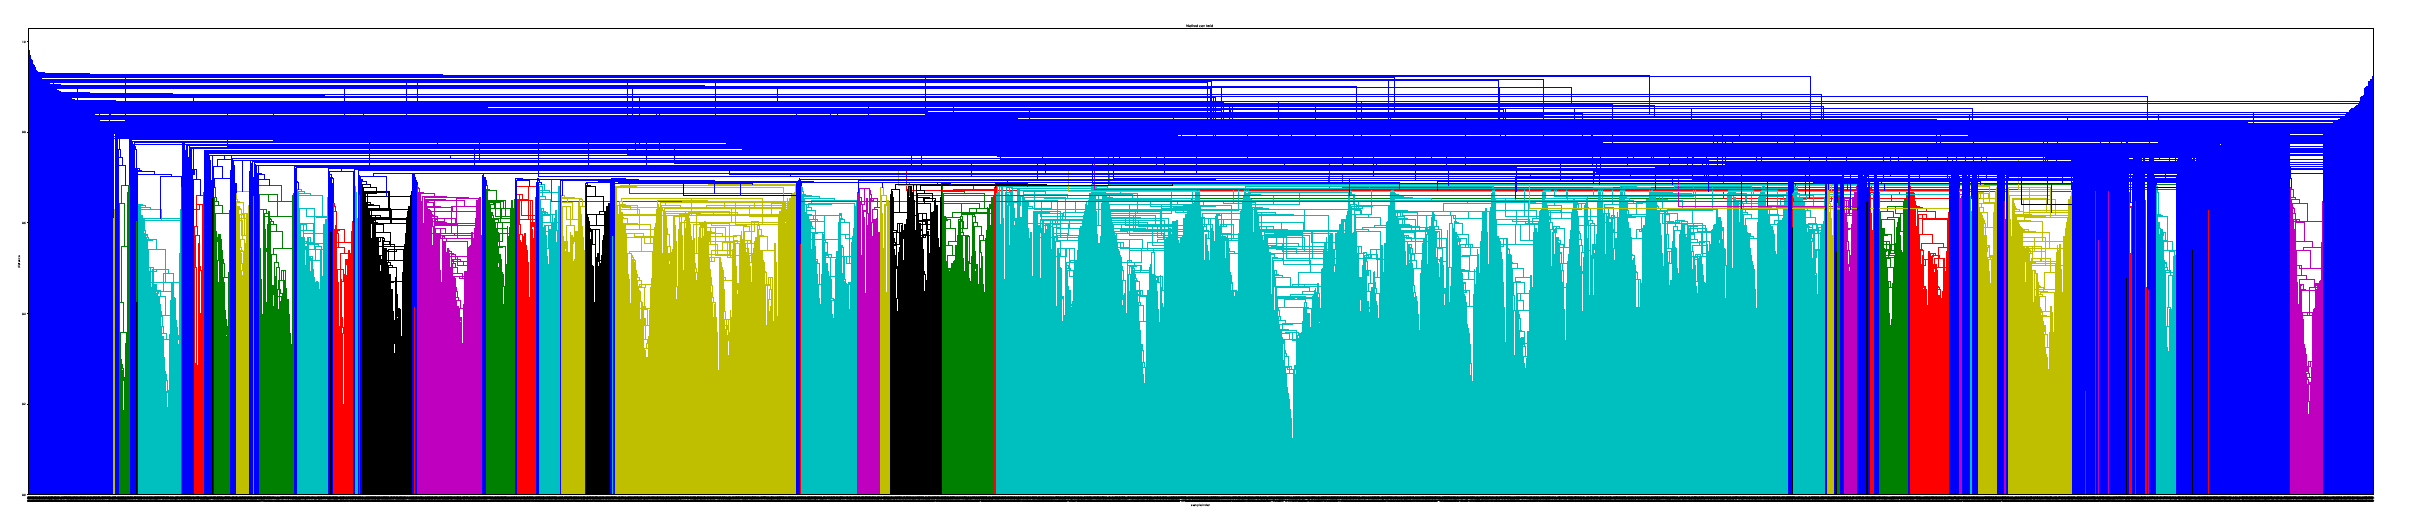
\includegraphics[width=16cm]{Figures/DendrogramAllDataset.png}
\caption{Dendrogram of all proposals.}
\label{fig:dendro.all}
\hfill
\end{figure}

An important feature of our dataset was that besides being small, the text was short. As Figure~\ref{fig:qty.words} shows, the majority of proposals have a length between 10 to 20 words per proposal (title + description), which is a clear limitation for our analysis.
Only few proposals have more than 30 words, this adds a challenge to the process of clustering similar proposals as it is more difficult to find similarities in short text as the co-occurrence of words decreased significantly when comparing to texts of hundreds of words. 

\begin{figure}[!htpb]
\begin{subfigure}{.5\textwidth}
  \centering
  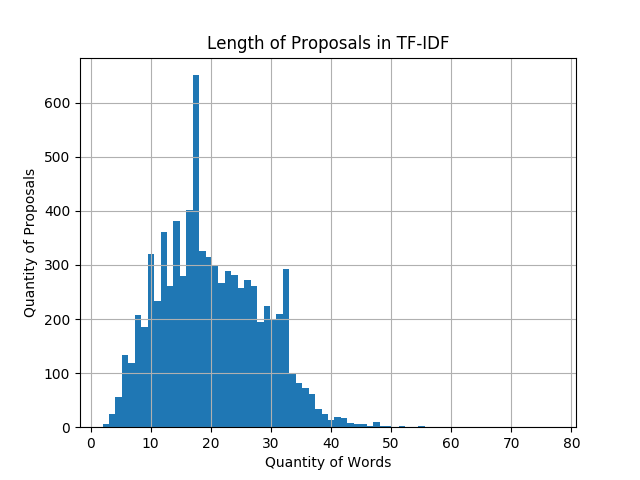
\includegraphics[width=8cm]{Figures/tfidf_words.png}
  \caption{}
  \label{fig:sub2}
\end{subfigure}
  \begin{subfigure}{.5\textwidth}
  \centering
  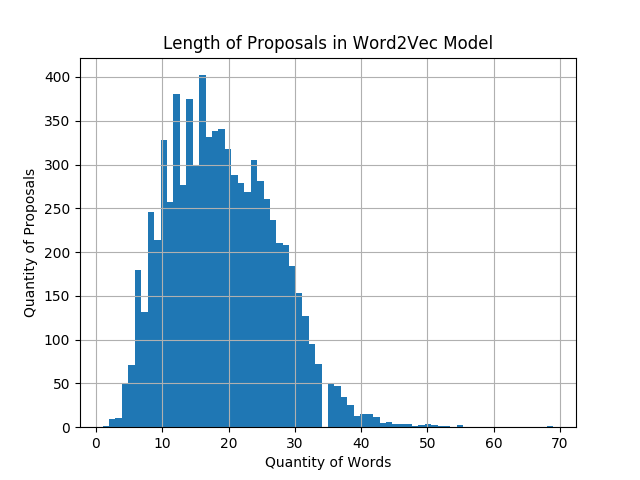
\includegraphics[width=8cm]{Figures/tfidf_word2vec_words.png}
  \caption{}
  \label{fig:sub3}
\end{subfigure}
\caption{Distribution of the number of words per proposal for two different representations. Most of the proposals have around 20 words, which is a limitation for our study.}
\label{fig:qty.words}
\end{figure}

\FloatBarrier
\section{Positive Results}
To achieve a result where external criterion output good values we had to change our approach. We decided to use a set of very different proposals and to use subcategories as our ground truth. We chose some proposals from very different subcategories to see which document representation gave the best result. The subcategories and distribution of proposals can be seen in table \ref{tab:mix.desc}. The content of these proposals is shown in table \ref{tab:positives}.

\begin{table}[!htpb]
\centering
{\scriptsize %
\begin{tabular}{l|c }
 \hline
Subcategories & Quantity\\
 \\\hline\hline 
Culture & 7  \\
Health & 15  \\
Host City & 7  \\
Sports &  12  \\
Transparent government   & 13\\
\hline
\end{tabular}
}%
\caption{Dataset description.}
\label{tab:mix.desc}
\end{table}

In table \ref{tab:negative.scores} we can see the best quality measures obtained from the clustering of the set of proposals from different subcategories using three different data representation; Tf-Idf, LSA and Word2Vec. We used different linkage methods, but only those that showed best results for at least one quality measure are shown in this section. Similarly, even when Euclidean distance was used for the experiments of this study, its results were in general worse than those obtained when using cosine distance. Therefore, we will limit the results of this chapter to those using cosine distance.

In table \ref{tab:mix.scores} we can notice that in general the three document representation used achieve good results. The main difference between this dataset and the global justice's dataset is that the classes in this one are highly different from one class to another making easier to divide proposals correctly. 
\begin{table}[!htpb]
\centering
{\scriptsize %
\begin{tabular}{c|c|c|c|c|c|c|c|c}
 \hline
Representation & Distance & Linkage & Cut Threshold & \#Clusters & NMI & Purity & ARI & Silhouette\\
\hline
\hline
\multirow{3}{*}{Tf-Idf}  & \multirow{3}{*}{Cosine}  & Complete & 0.0200 & 53 & 0.6279 & \textbf{1.0000}&  0.0055 & 0.0370 \\
 & & Average & 0.9400 & 6 & \textbf{0.8893} &  0.9630 & \textbf{0.8454} & 0.1113  \\
 & & Complete & 0.8000 & 26 & 0.6808 &  0.9630 & 0.1992 & \textbf{0.1711} \\
\cline{1-9}
\multirow{3}{*}{LSA}  & \multirow{3}{*}{Cosine}  & Complete & 0.0200 & 46 & 0.6426 & \textbf{1.0000}&  0.0431 & 0.2026 \\
 & & Complete & 0.7000 & 5 & \textbf{1.0000} &  1.0000 & \textbf{1.0000} & 0.6492  \\
 & & Average & 0.3600 & 5 & 0.9574 &  0.9815 & 0.9438 & \textbf{0.6638} \\
\cline{1-9}
\multirow{4}{*}{Word2Vec}  & \multirow{4}{*}{Cosine}  & Average & 0.4400 & 9 & \textbf{0.8972} & 1.0000 & 0.8105 & 0.1927 \\
 & & Complete & 0.0200 & 53 & 0.6279 & \textbf{1.0000}&  0.0055 & 0.0370 \\
 & & Average & 0.4400 & 9 & 0.8972 &  1.0000 & \textbf{0.8105} & 0.1927  \\
 & & Average & 0.5600 & 2 & 0.1029 &  0.2963 & 0.0086 & \textbf{0.2131} \\
\cline{1-9}
\hline
\end{tabular}
}%
\caption{Quality measures for subset of proposals from different categories.}
\label{tab:mix.scores}
\end{table}

Figure \ref{fig:mix.scores} shows the performance measured using purity, NMI, ARI and silhouette coefficient accross different number of clusters. For the three document representations is notable that at certain point (around 10 clusters) the highest score is achieved. In table \ref{tab:mix.scores} and figure \ref{fig:mix.scores} can be observed that NMI and ARI are maximized at the same number of cluster (actually implies the same cut threshold). This led us to think that combining more than one quality score can be more informative and helpful when deciding which is the best solution.

\begin{figure*}[!htp]
  \centering
    \vskip\baselineskip

  \begin{subfigure}[b]{0.49\textwidth}
  \centering
  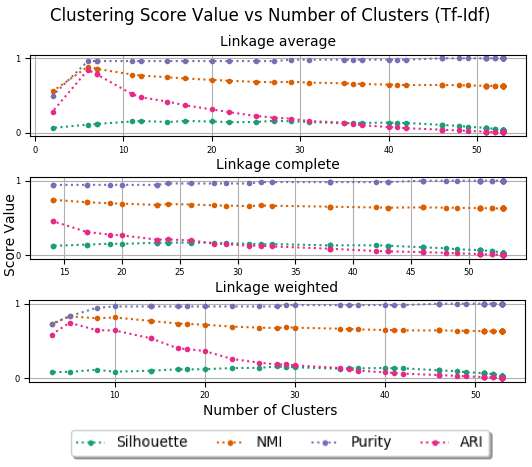
\includegraphics[width=\textwidth]{tfidf/clusters_score_tfidf_MIX.png}
  \caption[]%
  {{\small Tf-Idf.}}    
  \label{fig:mix.tfidf.score}
  \end{subfigure}
  \hfill
  \begin{subfigure}[b]{0.49\textwidth}  
  \centering 
  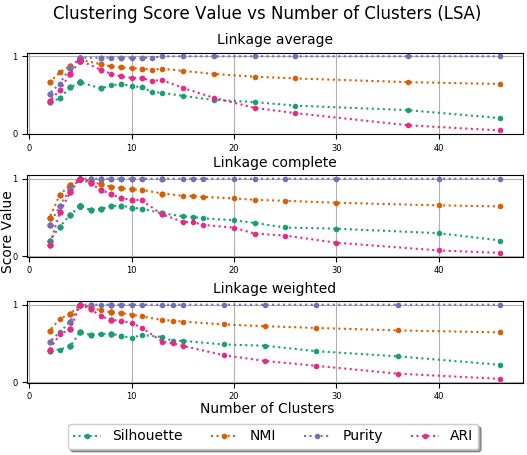
\includegraphics[width=\textwidth]{lsa/clusters_score_lsa_MIX.png}
  \caption[]%
  {{\small LSA.}}    
  \label{fig:mix.lsa.score}
  \end{subfigure}
  \hfill
  \end{figure*}
 \begin{figure*}[!htp]\ContinuedFloat
   \centering 
  \begin{subfigure}[b]{0.50\textwidth}   
  \vskip\baselineskip
  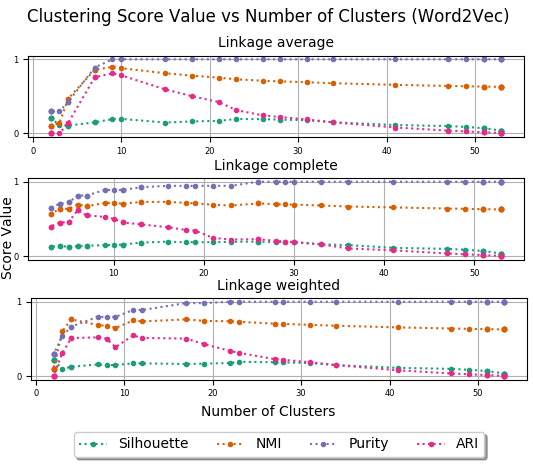
\includegraphics[width=\textwidth]{word2vec/clusters_score_word2vec_MIX.png}
  \caption[]%
  {{\small Word2Vec.}}    
  \label{fig:mix.word2vec.score}
  \end{subfigure} 
\caption{Quality measure results for Tf-Idf, LSA and Word2Vec of subset of proposals.}
\label{fig:mix.scores}
\end{figure*}

\FloatBarrier
\subsection{Tf-Idf Results}
In figure \ref{fig:mix.tfidf.dendro} we can see the dendrograms corresponding to the highest ARI and silhouette coefficient when using Tf-Idf over the proposals from different subcategories \ref{tab:mix.desc}. In these dendrograms we can observe that Tf-Idf success grouping proposals from same subcategories, this mainly product of the clearly different vocabulary used in each of these subcategories (see table \ref{tab:positives}).   
\begin{figure*}[!htpb]
  \centering
  \begin{subfigure}[b]{0.55\textwidth}  
  \centering 
  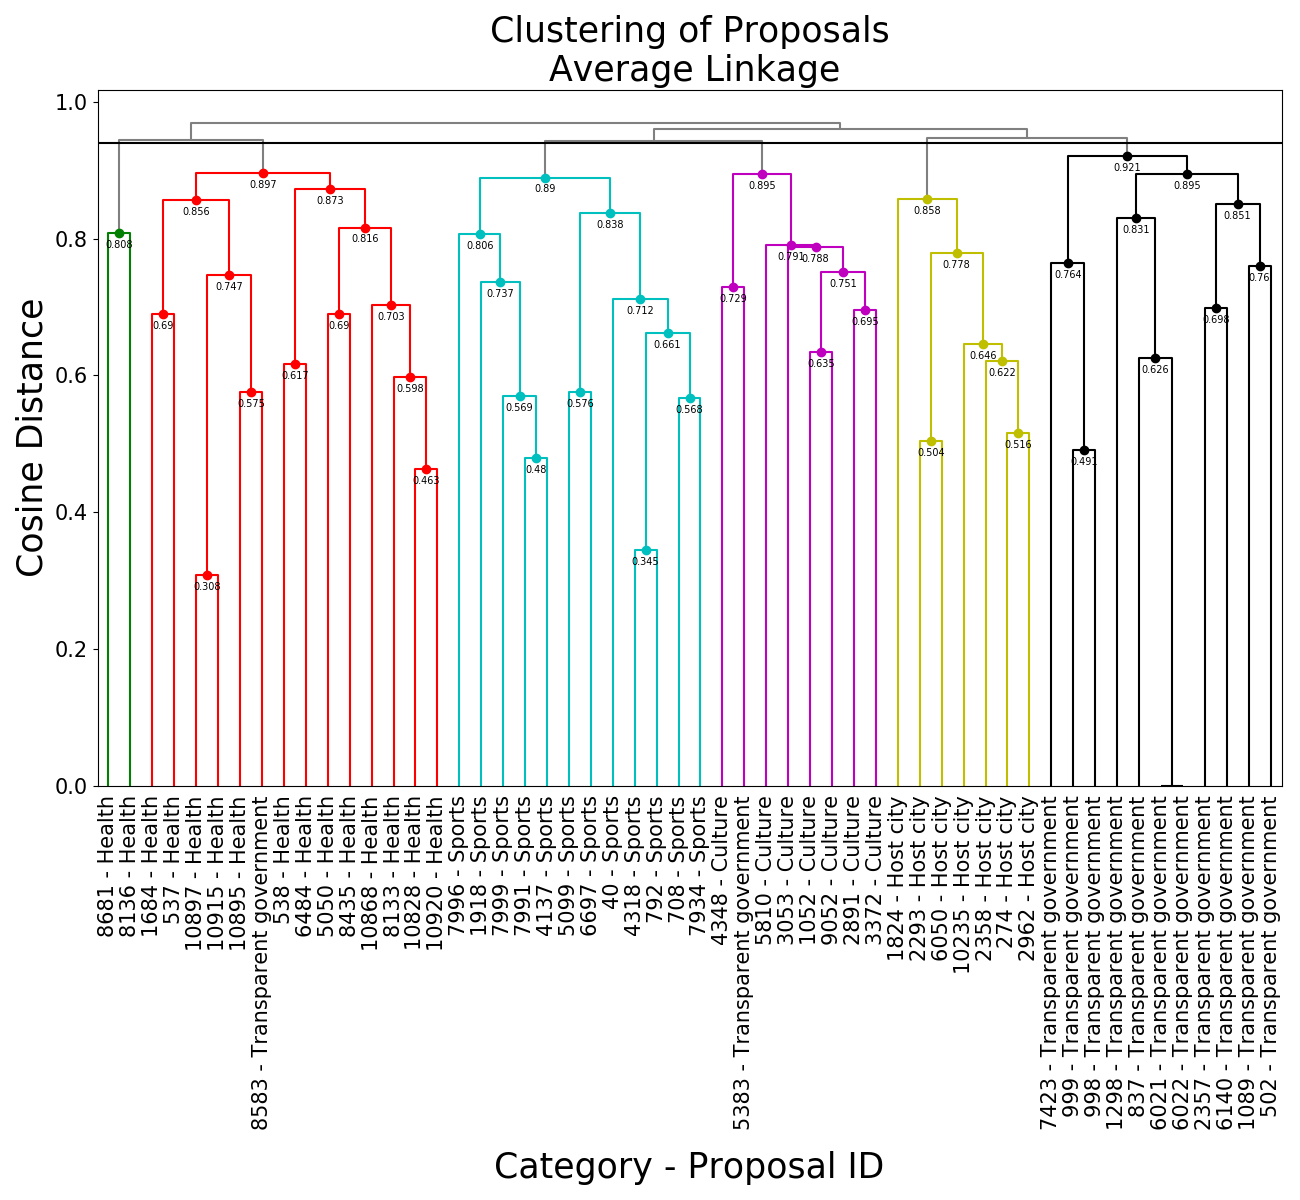
\includegraphics[width=\textwidth]{tfidf/BEST_ARI_MIX.png}
  \caption[]%
  {{\small Clustering with highest ARI.}}    
  \label{fig:mix.tfidf.ari.nmi}
  \end{subfigure}
  \begin{subfigure}[b]{0.55\textwidth}   
  \hfill
  \centering 
  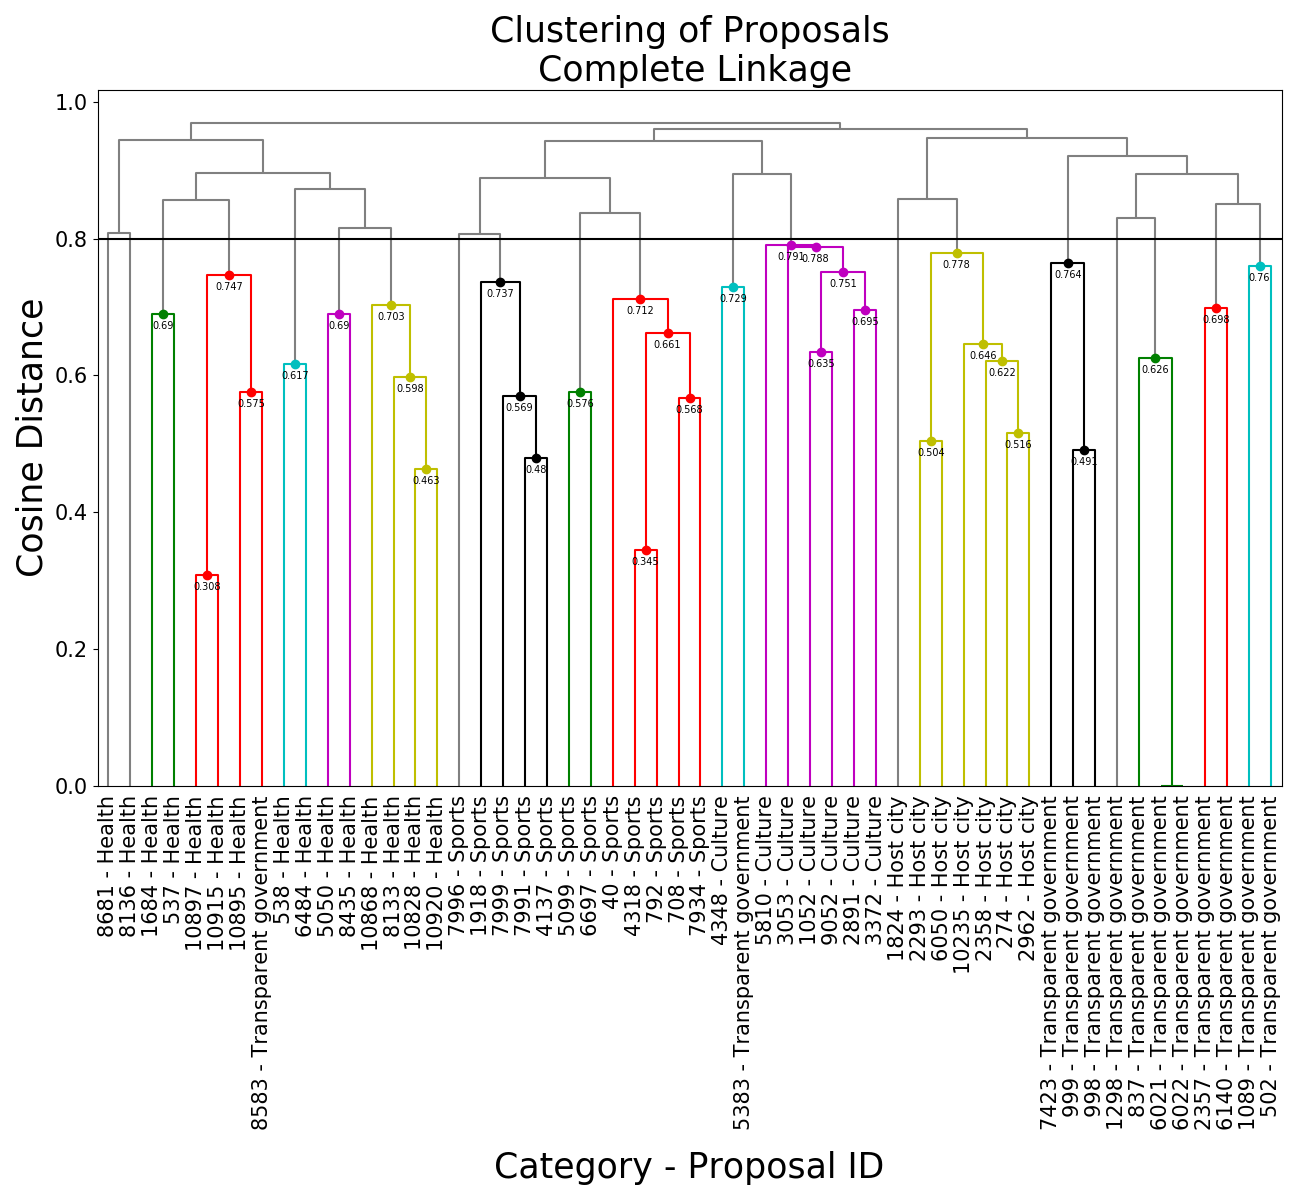
\includegraphics[width=\textwidth]{tfidf/BEST_SIL_MIX.png}
  \caption[]%
  {{\small Clustering with highest Silhouette.}}    
  \label{fig:mix.tfidf.sil}
  \end{subfigure}
\caption{Dendrogram with highest quality score of proposals from different categories (Tf-Idf).}
\label{fig:mix.tfidf.dendro}
\end{figure*}

\FloatBarrier
\subsection{LSA Results}
LSA gave of the best result from all the experiments carried over this dataset. We justify this by the difference of vocabulary between proposals of different subcategories; a property successfully caught by Tf-Idf. LSA improved Tf-Idf results by keeping more valuable features, removing all the noise captured by Tf-Idf. This can be clearly observed in the two dendrograms in figure \ref{fig:mix.lsa.dendro}.
\begin{figure*}[!htpb]
  \centering
  \begin{subfigure}[b]{0.55\textwidth}  
  \centering 
  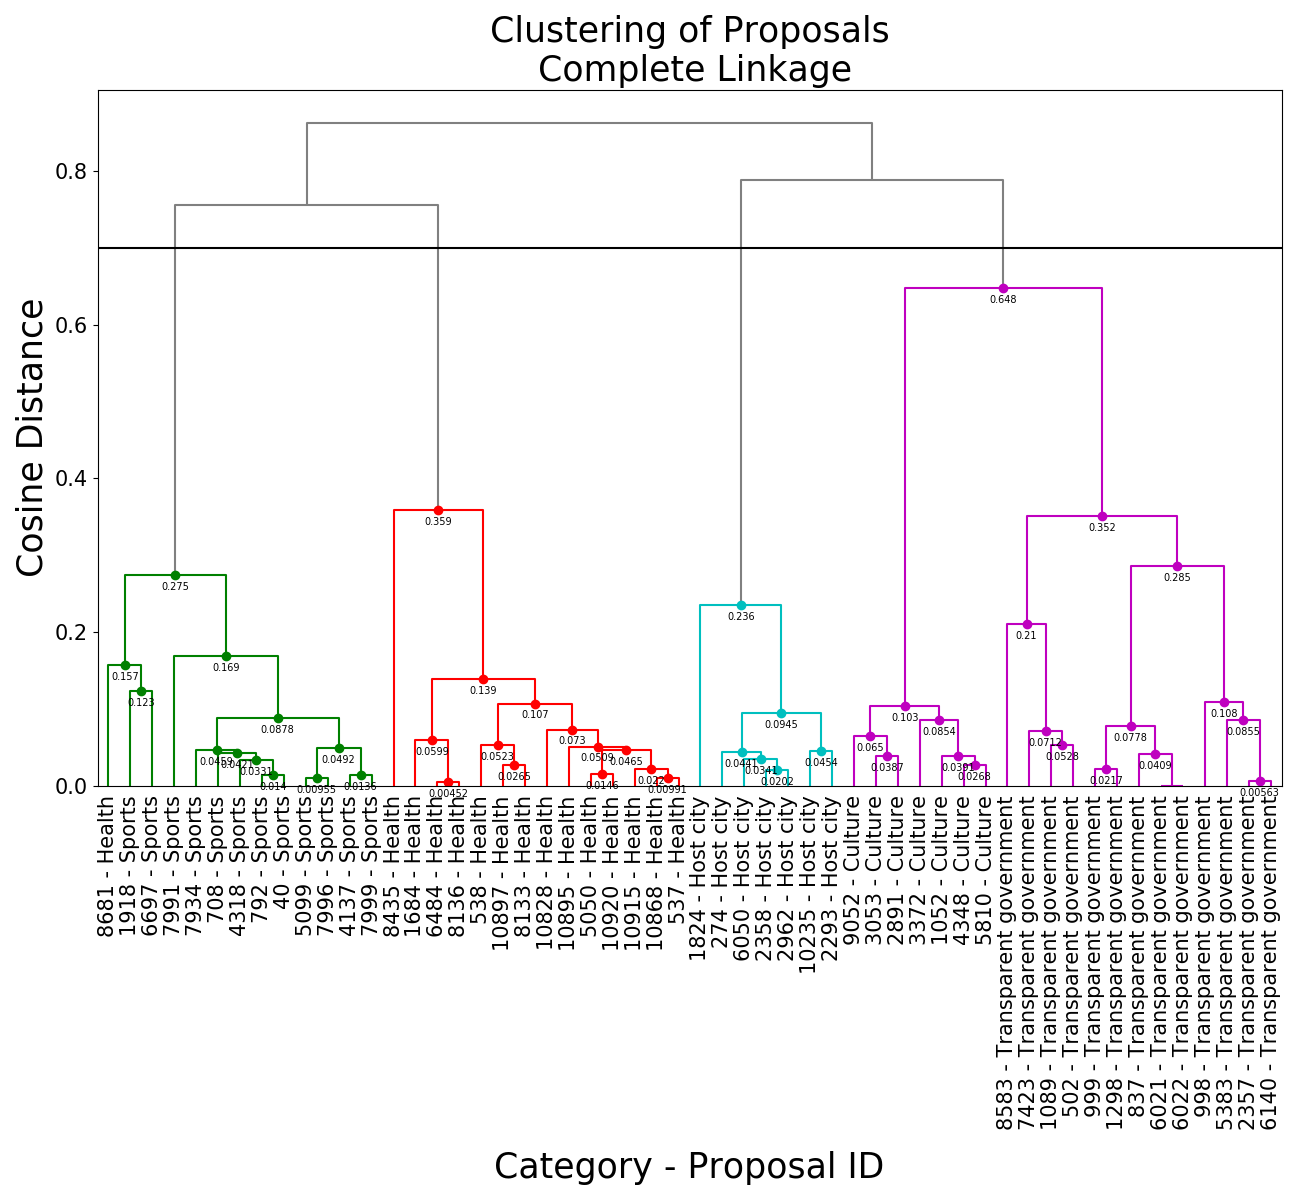
\includegraphics[width=\textwidth]{lsa/BEST_ARI_MIX.png}
  \caption[]%
  {{\small Clustering with highest ARI.}}    
  \label{fig:mix.lsa.ari}
 \end{subfigure}
 \end{figure*}

\begin{figure*}[!htpb]\ContinuedFloat
 \centering 
\begin{subfigure}[b]{0.55\textwidth}  
  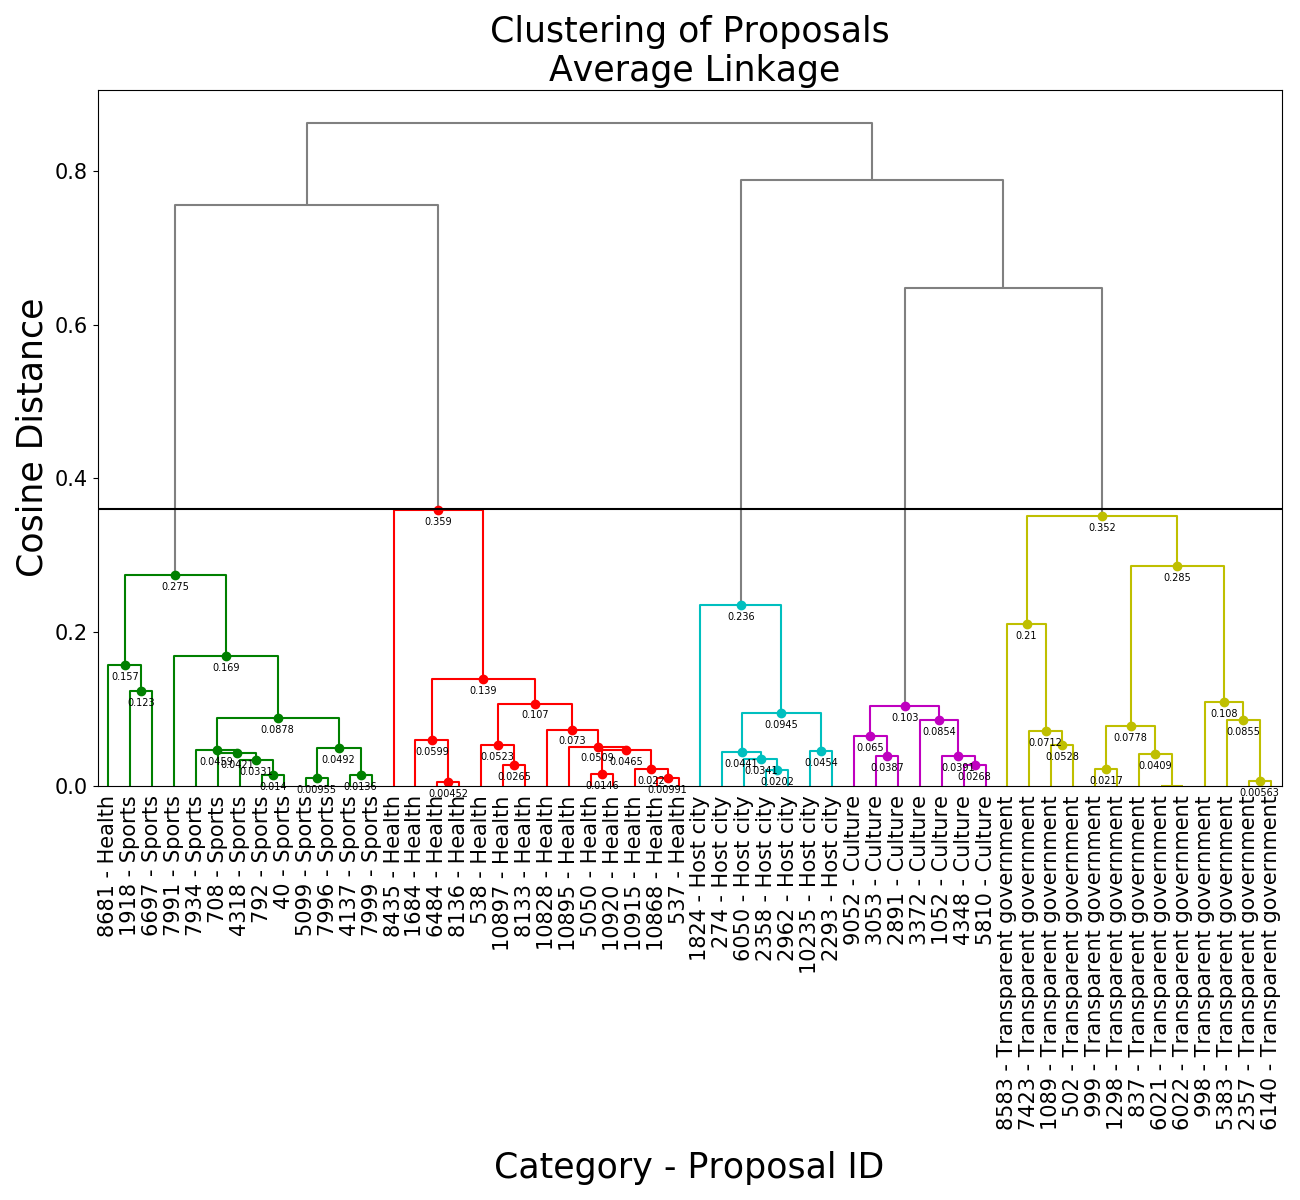
\includegraphics[width=\textwidth]{lsa/BEST_SIL_MIX.png}
  \caption[]%
  {{\small Clustering with highest Silhouette.}}    
  \label{fig:mix.lsa.sil}
  \end{subfigure}
\caption{Dendrogram with highest quality score of proposals from different categories (LSA).}
\label{fig:mix.lsa.dendro}
\end{figure*}

In figure \ref{fig:mix.lsa.ari} we see that the clusters obtained using LSA have a low intra-cluster distance and a high inter-cluster distance, what is a main goal when clustering data. This shows that LSA successfully groups this set of proposals.
\FloatBarrier
\subsection{Word2Vec Results}
Given the particularity of this dataset, already shown by Tf-Idf, it would have been surprisingly to find an extremely bad result in Word2Vec. We can see in figure \ref{fig:mix.word2vec.dendro} that Word2Vec is able to split the proposals into their subcategories, with only a few mistakes. Similarly to Tf-Idf, the clusters defined by Word2Vec are not compact, and the inter-cluster distance is relatively small, especially when compared to LSA results. This is caught by the best result of the silhouette coefficient, that given the high intra-cluster distance and the low inter-cluster distance found the best cut at 0.56 where the highest gap inter-clusters is reached. 
\begin{figure*}[!htpb]
  \centering 
  \begin{subfigure}[b]{0.59\textwidth}   
  \centering 
  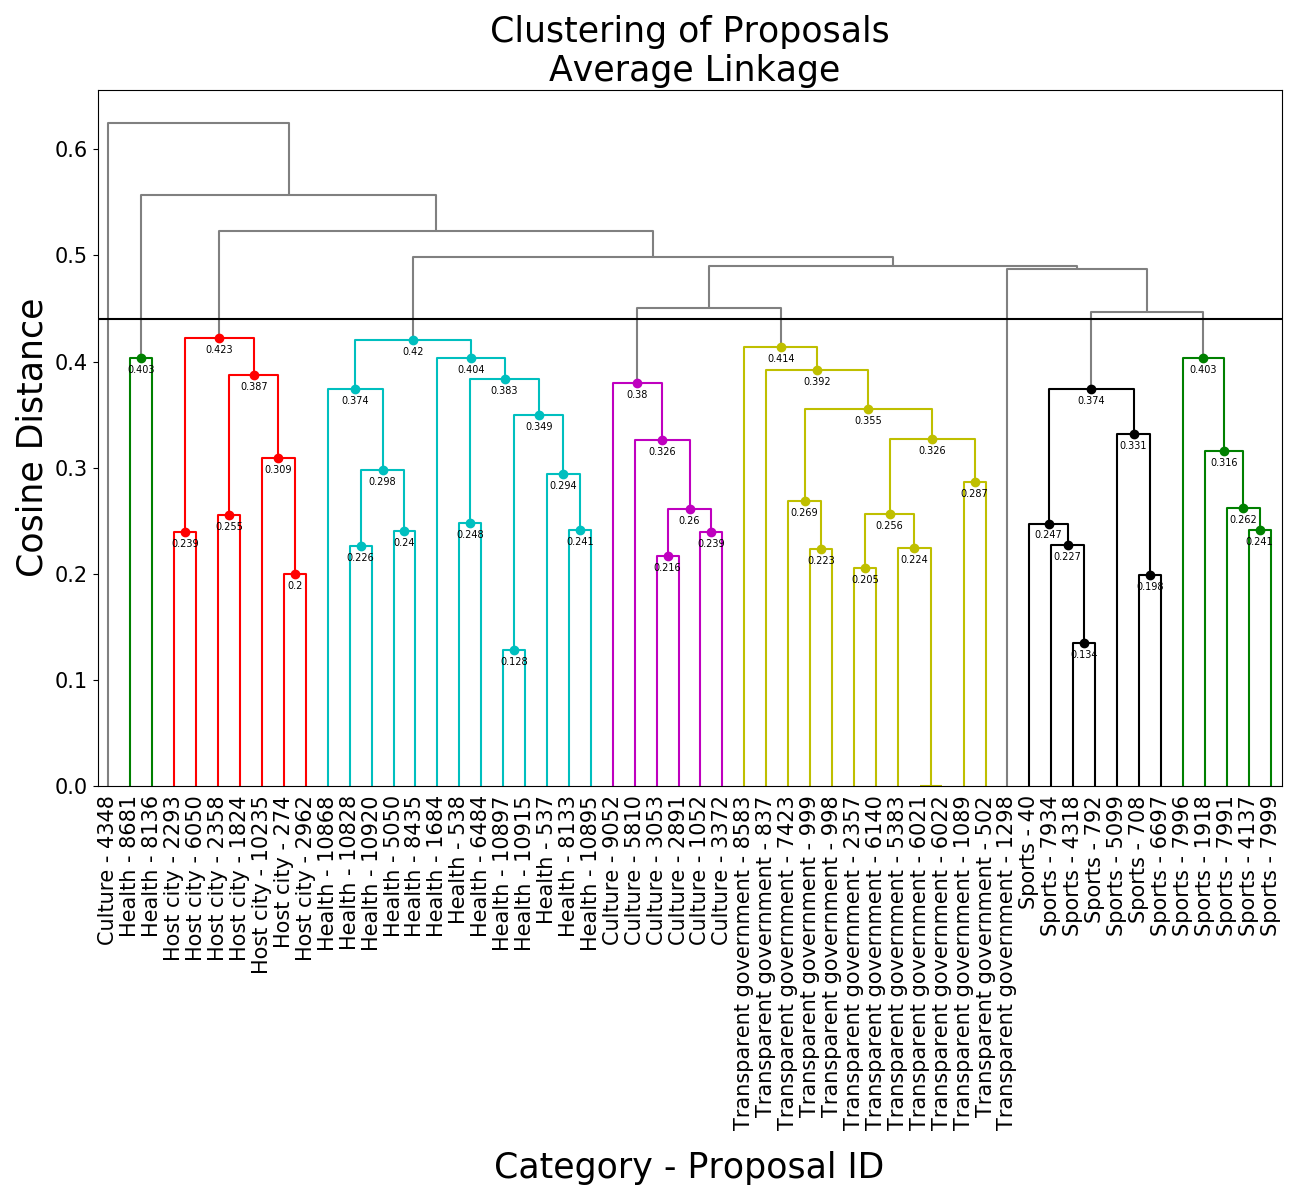
\includegraphics[width=\textwidth]{word2vec/BEST_ARI_MIX.png}
  \caption[]%
  {{\small Clustering with highest ARI.}}    
  \label{fig:mix.word2vec.ari}
  \end{subfigure}
  \hfill
  \centering 
  \begin{subfigure}[b]{0.59\textwidth}   
  \centering 
  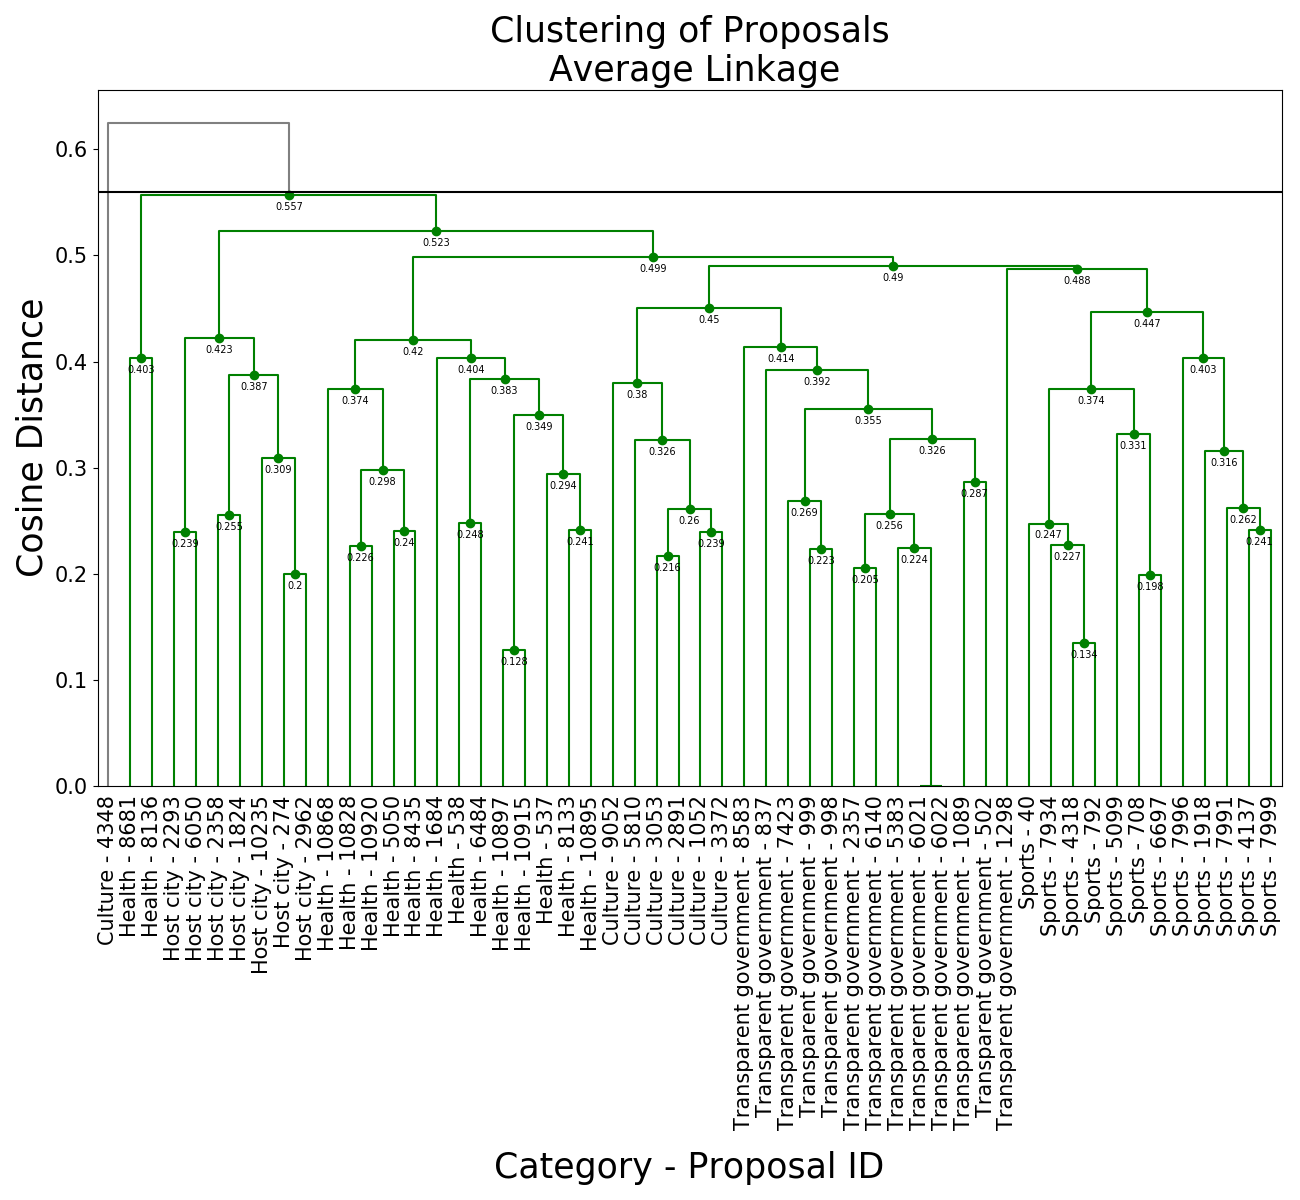
\includegraphics[width=\textwidth]{word2vec/BEST_SIL_MIX.png}
  \caption[]%
  {{\small Clustering with highest Silhouette.}}    
  \label{fig:mix.word2vec.sil}
  \end{subfigure}
\caption{Dendrograms with highest quality score of proposals from different categories (Word2Vec).}
\label{fig:mix.word2vec.dendro}
\end{figure*}
    
\FloatBarrier

\scriptsize %%%%%%%%%%%  smaller font size %%%%%%%%
\begin{spacing}{1}
\begin{longtable}{m{30mm}|m{85mm}|c|m{15mm}}
\hline
Title & Description & Proposal & Category  \\
\hline
\hline
\endhead
 Visibilize the cultural activities of the district in the city circuit & Promote proposals and cultural productions that take place in Nou Barris and propose one of these projects in the city to enter the cultural map of Barcelona. & 1052 & Culture  \\ \hline
 Open the exhibition spaces of the district to the entities and the neighborhood of the territory & Generate competition bases to open the four exhibition halls of the city to all kinds of proposals, to turn them into spaces to promote popular and cultural exhibits, as well as personal artistic proposals. & 3053 & Culture  \\ \hline
 Promote the participation of the families of students in cultural activities & Promote the participation of the families of students in cultural activities. & 9052 & Culture  \\ \hline
 Commercial axis as a vehicle for cultural dissemination & Commercial axis: entities and stores as vehicles of cultural dissemination The dissemination can be done through the shops & 4348 & Culture \\ \hline
 Coordination of the networking of large cultural facilities and those with entities, communities and collectives, both in the cultural and academic worlds & Encourage networking and new collaborative projects between libraries, civic centers, cultural entities, large museums or research and creation spaces to ensure the maximum circulation of contents and artistic practices. & 2891 & Culture \\ \hline
 Coordination of the city's culture & Create a brand that coordinates the entire cultural offer in Barcelona, ​​both from public and private entities. & 3372 & Culture \\ \hline
 The libraries of the District as cultural agents of knowledge of the territory. & Activities organized by the libraries and other entities to make known the Heritage and the History of the District to the users. & 5810 & Culture \\ \hline
 Day We create health to reduce inequalities: Go to the causes of causes. & To give importance to the diagnoses to go to the causes of the causes. & 10897 & Health \\ \hline
 Mental health improvement projects & Encourage projects of entities in the sector to improve the mental health of the population. & 538 & Health \\ \hline
 Strengthen the network of Mental Health for children and adolescents & Strengthen the network of Mental Health for children and adolescents to support situations of crisis and consultation in schools and caregivers.To attend more quickly and to prioritize infant at high risk. & 6484 & Health \\ \hline
 Mental Health Plan: Support programs for professionals. & Training and specific resources for professionals in childhood and adolescence.Areas of coordination and work with young and homeless spaces. & 10828 & Health \\ \hline
 Speeches of talks by neighborhoods of health professionals & Make a talk series of health professionals with entities, Neighborhood Associations etc.To improve the information. & 8133 & Health \\ \hline
 Day We create health to reduce inequalities: symbiotic interventions. & Symbiotic interventions where different populations and needs benefit mutually from their strengths, being voluntary or new sources of employment. & 10915 & Health \\ \hline
 Health in Barcelona: Review the patient care model. & To train professionals from the empowerment model.Go from the assistance model to an empowering model.Do not generate employee dependence. & 10868 & Health \\ \hline
 Day We create health to reduce inequalities: More resources are needed so that professionals can do more work and community actions. & For example, more home care, street work, community mediation, etc ...). & 10895 & Health \\ \hline
 Increase medical assistance - Horta Guinardó. & It is proposed to increase the number of doctors to offer a better medical assistance service, especially in general medicine. & 8681 & Health \\ \hline
 Reopen / create the services previously referred to as 'family planning' & The life cycle of women has sexual characteristics specific to the potential and / or reproductive activity: menstruation, pregnancy, menopause are phases, not diseases, which should be able to monitor proximity to all neighborhoods.Women's sexual health centers would be very useful. & 1684 & Health \\ \hline
 Training in health workers in functional diversity & Training health workers as gynecologists in functional diversity so that they can break a little with the taboos of this group and be able to accompany them in a more integral way & 5050 & Health \\ \hline
 Ensure the existence of quality public services and specific services for young people, incorporating a gender perspective and respect for affectivosexual diversity, both in primary care centers and in educational centers & Promotion of training from the ASPB to professionals in the field of medicine, especially those that work around the ASSiR in LGBTI issues, gender perspective, sexual diversity Maintain and expand the specialized care services of the young people taking into account gender perspective, gender and sexual diversity within the CAPs. & 8435 & Health \\ \hline
 Training in interculturality for health professionals. & Training in interculturality for health professionals. & 10920 & Health \\ \hline
 Comprehensive community health plan, women, the elderly and the immigrant population & Create a Health Table equipped with your own resources & 537 & Health \\ \hline
 Guarantee the stability of budgets and recovery of health services and outsourced services: & Recover all those sanitary services that have been eliminated due to the cuts and all the services that have been derived to private entities.https://decidim.barcelona/proposals/reduccio-de-les-externalizaciones-i-les-privatizaciones-de-serveis-sanitaris & 8136 & Health \\ \hline
 Incorporate LGBT perspective in the refugee support plan & Incorporate the LGTBI perspective in the refugee support plan and take into account its rights as LGBT people. & 10235 & Host city \\ \hline
 Initiatives with refugees. & creation of shelters, reception. & 2293 & Host city \\ \hline
 Attention to refugees. & Barcelona City Refuge, neighborhood committed to the refugees, platform creation or support group & 2358 & Host city \\ \hline
 Start the "Refuge" plan & The District of the Eixample undertakes to develop the "Refuge" plan and to promote the involvement of entities and groups in the different neighborhoods in this plan. & 274 & Host city \\ \hline
 Start the plan "Barcelona, ​​a city refuge" & Start up an operational and strategic plan for the reception of the city.To create a stable and permanent support structure for refugees and asylums that is complementary to state programs, with their own criteria and in collaboration with entities that work on the subject.Pay special attention to asylum seekers who are left out of the state social support program.Create a city-to-city cooperation plan for the high-density municipalities receiving refugees and migrants. & 2962 & Host city \\ \hline
 Participation in the Social Area Barcelona City Refuge & Participation in the Social Area Barcelona City Refuge & 1824 & Host city \\ \hline
 Create a bank of resources for refugees at the level of the District connected to the Generalitat in two levels (reception and awareness) & The reception of refugees in the city must be planned, work in conjunction with the Generalitat and establish measures to: - The reception (accommodation, support, language, etc.) - Awareness (educational centers and citizenship in general) & 6050 & Host city \\ \hline
 Installation of gymnastics devices in the public parks of La Marina - Zona Franca. & Promote young people's sports practice. & 4318 & Sports \\ \hline
 Comprehensive reform of the Municipal Narcís Hall Camp & Continue with the process of integral reform of the Narcí Sala Municipal Camp and execute phases 2, 3 and 4 during the years 2016, 2017 and 2018 respectively.This process will always count with the participation and supervision of the managing entity, which will also be revamped with provisional facilities while the works affect parts of the stadium. & 1918 & Sports \\ \hline
 Take advantage of the dimensions of the old soccer field in Santander street for sports that require large sizes & and avoid dividing it into small clues, since the opportunity that this great space is giving away is wasted & 5099 & Sports \\ \hline
 Coherence in municipal sports facilities with the environmental policies promoted by the City Council. & Be consistent in sports facilities with the policies promoted by the City Council, especially with the selective collection of waste. & 7991 & Sports \\ \hline
 Encourage sports programs for children and young people during the holiday season & Promote sports practice during holiday periods, in order to guarantee the rights to the access and the sporting practice of young people and children, regardless of their conditions and the territory in which they live, and to promote the reconciliation of family life. & 792 & Sports \\ \hline
 Creation of sports and play areas in the public space & Generate new areas of sports and play areas in the public space in order to promote a healthy, active and community life. & 708 & Sports \\ \hline
 Create a sports area for young people in the Free Trade Zone & In the face-to-face event that took place at the IES Montjuïc, the 4th ESO students proposed the creation of a sports area for young people in the Free Trade Zone & 7934 & Sports \\ \hline
 Adapt the maintenance of sports spaces to the volume of users. & In order to guarantee the proper maintenance of the equipment, adapt it to the volume of use of the equipment.Track in a specific and adapted way to each facility.Especially in the summer season. & 7996 & Sports \\ \hline
 Improve and transfer sports spaces & It is valued to promote health from these entities through the availability of these spaces.They put the example of the chromium of the youth house of the courts, which should be improved and give way to the football field & 6697 & Sports \\ \hline
 Children's Sports Festival & Promote the Children's Sports Festival as a showcase for sports activities and the different sports groups of Gràcia.Promote the participation of schools and school sports. & 40 & Sports \\ \hline
 Open more municipal sports facilities. & Open more municipal sports facilities.In the case of Poble Nou, they can only access Can Felipa, who perceive that it is saturated and has limited and inadequate facilities. & 4137 & Sports \\ \hline
 Reduction and adaptation of the quotas for municipal sports facilities. & Reduce access prices to municipal sports facilities.Adapt the quotas to the different groups, make specific quotas for families, large families, retirees, and other groups.Set the hour division into two strips.Universalise the price of the equipment.Flexible quotas to include a minimum service of activities. & 7999 & Sports \\ \hline
 Encourage and increase municipal information & Support the radio of Sants.To make campaigns for the dissemination and awareness of participation.Increase political transparency.More understandable information for citizens, nearby. & 5383 & Transparent government \\ \hline
 To achieve the full transparency and retention of accounts of public management & Recognize and facilitate the work of popular control initiatives, such as citizen observatories against corruption, transparency and good governance and promote a citizen advice that audits the proceedings of the district. & 6021 & Transparent government \\ \hline
 Prepare the District Transparency Plan & Design and launch a plan with information that is neat and easy to consult through the Internet, which allows you to know in detail the budgets, the use made of the public resources and the actions carried out by the Administration and its institutional representatives. & 1089 & Transparent government \\ \hline
 To achieve the full transparency and retention of accounts of public management & Recognize and facilitate the work of popular control initiatives, such as citizen observatories against corruption, transparency and good governance and promote a citizen advice that audits the proceedings of the district. & 6022 & Transparent government \\ \hline
 Change how the City Council operates internally on some fronts linked to the common good: strengthen the existing procommun communities, respecting their autonomy & As a general principle, support communities of the existing procommunication and / or technologies, instead of replacing them with the administration, promoting the consolidation or creation of communities that can be self-managed and allow them to be autonomous, They respect ethical questions and work for the common good. & 7423 & Transparent government \\ \hline
 Improvement in communication channels with the City Council. & Parity work sessions, e-Government, Open Data, Technology and politics, e-voting, information on right access to information, web where citizens can propose projects. & 2357 & Transparent government \\ \hline
 Develop an ethical code for elected officials and management personnel & Develop the code that aims to establish the principles and ethical values ​​and the rules of conduct that must be respected by the elected officials and municipal management personnel in the exercise of their functions, with the main purpose of guaranteeing efficient, complete management and transparent from the municipal administration. & 999 & Transparent government \\ \hline
 Enable an ethical mailbox & Enabling an ethical mailbox conceived as a tool for participation so that citizens can safely communicate to the City Council facts and behaviors that are contrary to an ethical management of the Administration. & 998 & Transparent government \\ \hline
 Portal of transparency & Publish the councilor's agenda, as well as its declaration of assets and interests;The declarations of goods and interests of District Counselors will also be published, and the District's estimates and investments will be made public. & 837 & Transparent government \\ \hline
 District communication plan & Write and execute the Communications Plan of the District of the Cortes in order to improve the tools that give logic, coherence, purpose and effectiveness to internal and external communication. & 502 & Transparent government \\ \hline
 Improve the information and accessibility of the websites of the City Council & Facilitate the knowledge of the activities, actions of the city council.Improve transparency. & 6140 & Transparent government \\ \hline
 Improve general communication and transparency on ongoing works and on the street & I still see works every day without knowing what they are doing (eg, a type of orchard street Mare de Deus de las Neus, we have a look at it from home, we do not know after 2 years that it is neither for whom). They still continue to do the works clear poster that announces that something will be done soon, for whom, the final result, the financing. & 8583 & Transparent government \\ \hline
 waiting room for saints & The Citizen Attention Office dl district of Sants has a ludic waiting room for the large number of citizens who are going to take steps.There is no maximum capacity or limit.There are also windows and therefore not natural light.There is air conditioning but when there are so many people in the summer it is not noticeable.It's small and claustrophobic.You need a larger room & 1298 & Transparent government \\ \hline

\caption{Set of correctly clustered proposals.}
\label{tab:positives} \\
\end{longtable}
\end{spacing}
\normalsize

\FloatBarrier
\section{Negative Results}

The results presented in this section correspond to Global Justice's proposals. This category has a total of 45 accepted proposals \ref{tab:data.desc}. Actuations (also called results) are composed by one to many proposals. From the 45 global justice's proposals we will use only the 29 proposals that are within an actuation of more than one proposal. For details of the content of these proposals look at table \ref{tab:negatives}.

% Proposals in the category of global justice tackle these main subjects: Refugees, human rights, migrants, international networking, international cooperation. After reading the proposals in \ref{tab:data.desc} we could naturally group proposals as follow (for space reasons we will show the proposals Id):
% \begin{itemize}
% \item Refugees: 2293, 2358, 6142, 
% \end{itemize}

In table \ref{tab:negative.scores} we can see the best quality measures obtained from the clustering of global justice's proposals using Tf-Idf, LSA and Word2Vec.


\begin{table}[!htpb]
\centering
{\scriptsize %
\begin{tabular}{c|c|c|c|c|c|c|c|c}
 \hline
Representation & Distance & Linkage & Cut Threshold & \#Clusters & NMI & Purity & ARI & Silhouette\\
\hline
\hline
\multirow{4}{*}{Tf-Idf}  & \multirow{4}{*}{Cosine}  & Complete & 0.4606 & 26 & \textbf{0.7068} & 0.9655 & 0.0344 & 0.0880 \\
 & & Complete & 0.2206 & 28 & 0.6965 & \textbf{0.9655}&  -0.0049 & 0.0489 \\
 & & Average & 0.8806 & 4 & 0.4991 &  0.5517 & \textbf{0.3399} & 0.1163  \\
 & & Complete & 0.9006 & 10 & 0.6183 &  0.7241 & 0.2152 & \textbf{0.1879} \\
\cline{1-9}
\multirow{4}{*}{LSA}  & \multirow{4}{*}{Cosine}  & Complete & 0.0371 & 26 & \textbf{0.6660} & 0.8966 & -0.0144 & 0.1544 \\
 & & Complete & 0.0371 & 26 & 0.6660 & \textbf{0.8966}&  -0.0144 & 0.1544 \\
 & & Average & 0.7171 & 3 & 0.3521 &  0.5172 & \textbf{0.2711} & 0.4137  \\
 & & Average & 0.4371 & 5 & 0.4476 &  0.5862 & 0.1949 & \textbf{0.5899} \\
\cline{1-9}
\multirow{4}{*}{Word2Vec}  & \multirow{4}{*}{Cosine}  & Complete & 0.1577 & 27 & \textbf{0.7016} & 0.9655 & 0.0149 & 0.0498 \\
 & & Complete & 0.0977 & 28 & 0.6965 & \textbf{0.9655}&  -0.0049 & 0.0337 \\
 & & Average & 0.5177 & 4 & 0.4367 &  0.5517 & \textbf{0.1652} & 0.2890  \\
 & & Average & 0.5977 & 2 & 0.1123 &  0.4138 & 0.0033 & \textbf{0.3491} \\
\cline{1-9}
\hline
\end{tabular}
}%
\caption{Quality measures for Global Justice's Proposals.}
\label{tab:negative.scores}
\end{table}

In figure \ref{fig:gj.scores} we can see the behavior of the four scores used to measure the quality of our output. We can see how purity and NMI tend to favor those result with a higher number of clusters. For this subset of proposals we found more reliable to use ARI and Silhouette coefficient to decide which would be the best clustering results, as both of them do not favor solutions with high cardinality.
% To find an appropriate measure to evaluate the goodness of our results was extremely challenged. We tested some of the measures available and widely use, and their drawbacks make difficult to chose the best result only by looking at the best score. 
\begin{figure*}[!htp]
  \centering
  \begin{subfigure}[b]{0.49\textwidth}
  \centering
  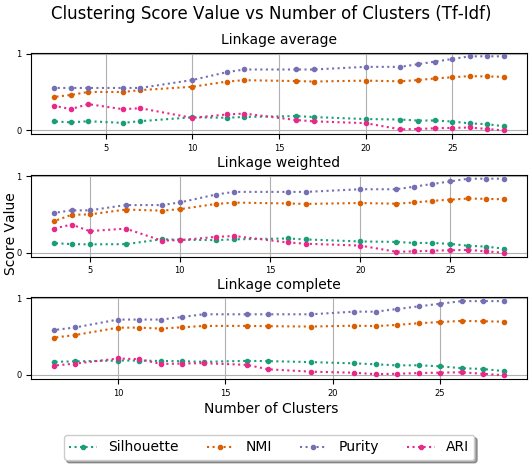
\includegraphics[width=\textwidth]{tfidf/clusters_score_tf-idf_Global_Justice.png}
  \caption[]%
  {{\small Tf-Idf.}}    
  \label{fig:gj.tfidf.score}
  \end{subfigure}
  \hfill
  \begin{subfigure}[b]{0.49\textwidth}  
  \centering 
  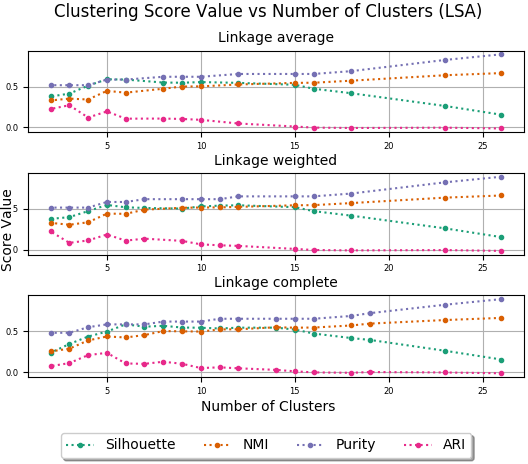
\includegraphics[width=\textwidth]{lsa/clusters_score_lsa_Global_Justice.png}
  \caption[]%
  {{\small LSA.}}    
  \label{fig:gj.lsa.score}
  \end{subfigure}
  \vskip\baselineskip
 
  \begin{subfigure}[b]{0.49\textwidth}   
  \centering 
  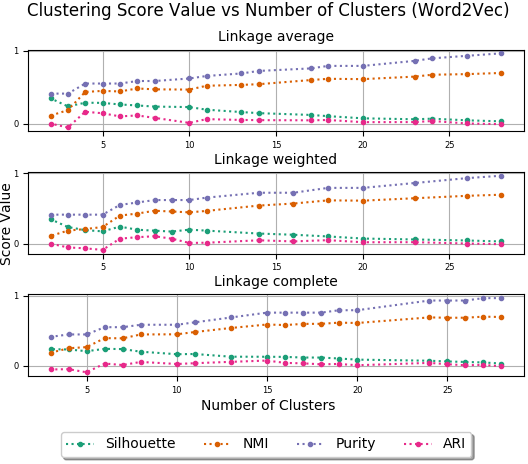
\includegraphics[width=\textwidth]{word2vec/clusters_score_word2vec_Global_Justice.png}
  \caption[]%
  {{\small Word2Vec.}}    
  \label{fig:gj.word2vec.score}
  \end{subfigure} 
\caption{Quality measure results for Tf-Idf, LSA and Word2Vec of Global Justice's Proposals.}
\label{fig:gj.scores}
\end{figure*}

The original number of classes of global justice's proposals is seven. In table \ref{tab:negative.scores} we can see that none of the best scores results in this number of clusters. The closest clustering result was the obtained by using LSA + Average Linkage. However, the obtained clustering in this case does not agree with our ground truth, as ARI shows. Nevertheless, the resulting clustering shows a high silhouette coefficient, and giving the fact that our ground truth was not totally reliable, we tend to trust in results with high silhouette coefficient, this shows that the proposals in each cluster are very similar between then and clearly different from proposals in other clusters. 
\FloatBarrier
\subsection{Tf-Idf Results}
Looking at table \ref{tab:negative.scores} we will automatically discards the results where the dendrogram is cut at 0.4606 and 0.2206 (see Figure \ref{fig:gj.tfidf.nmi} and \ref{fig:gj.tfidf.purity} respectively), there can be seen that this result show not useful clusters. The solutions with the closest number of clusters to the actual number of classes are the one from using average linkage and cutting the dendrogram at 0.9006. In \ref{fig:gj.tfidf.ari} can be seen 4 clusters, which any of then perfectly matching the ground truth, however, looking at the content of the proposals for each of these clusters it is evident that at least 3 of these 4 clusters have a clear tendency to group proposals that tackle the main topic. From \ref{fig:gj.tfidf.ari}) we can see these topics:
\begin{enumerate}[itemsep=1pt,parsep=1pt]
\item Green cluster: Global justice, international network.
\item Red cluster: International cooperation, exchange of practices across cities.
\item Blue cluster: Refugees.
\item Purple cluster: This is the least clear, it mainly talks about specific cities in the Mideast, humanitarian crisis and refugees.
\end{enumerate}
From the above results, we can conclude that, even when the clustering was not perfect, specially compared to the ground truth, in general proposals that have similar words were in the same cluster. This result is what we expected from Tf-Idf, which is good at finding proposals that have word overlapping.

\begin{figure*}[!htpb]
  \centering
  \begin{subfigure}[b]{0.48\textwidth}
  \centering
  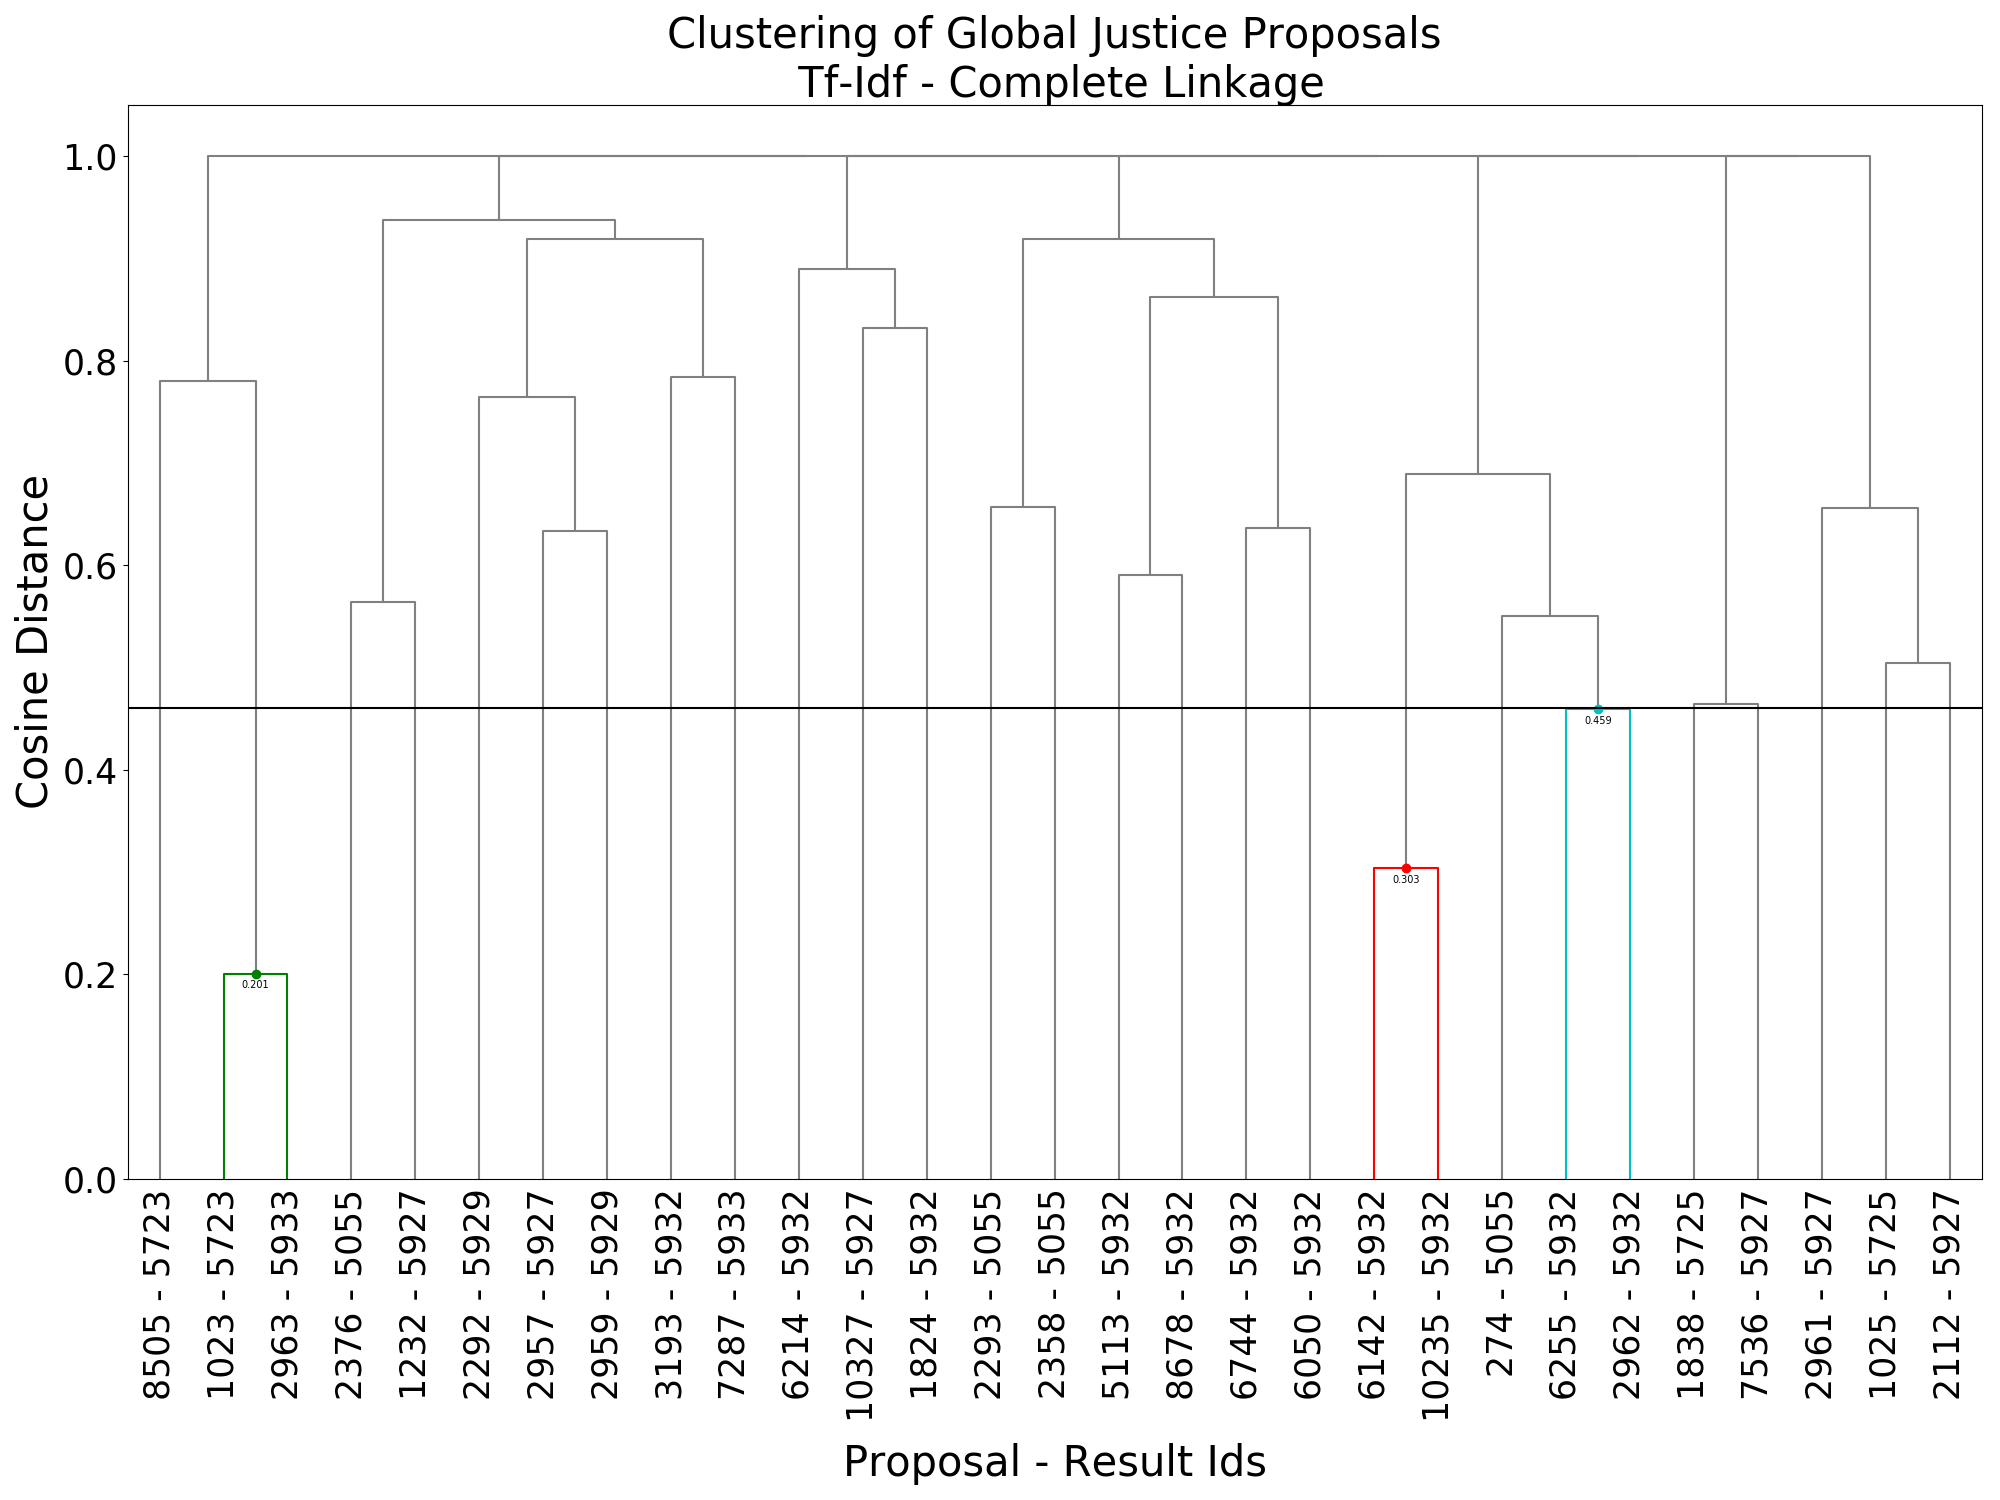
\includegraphics[width=\textwidth]{tfidf/BEST_NMI_Global_Justice.png}
  \caption[]%
  {{\small Clustering with highest NMI.}}    
  \label{fig:gj.tfidf.nmi}
  \end{subfigure}
  \hfill
  \begin{subfigure}[b]{0.48\textwidth}  
  \centering 
  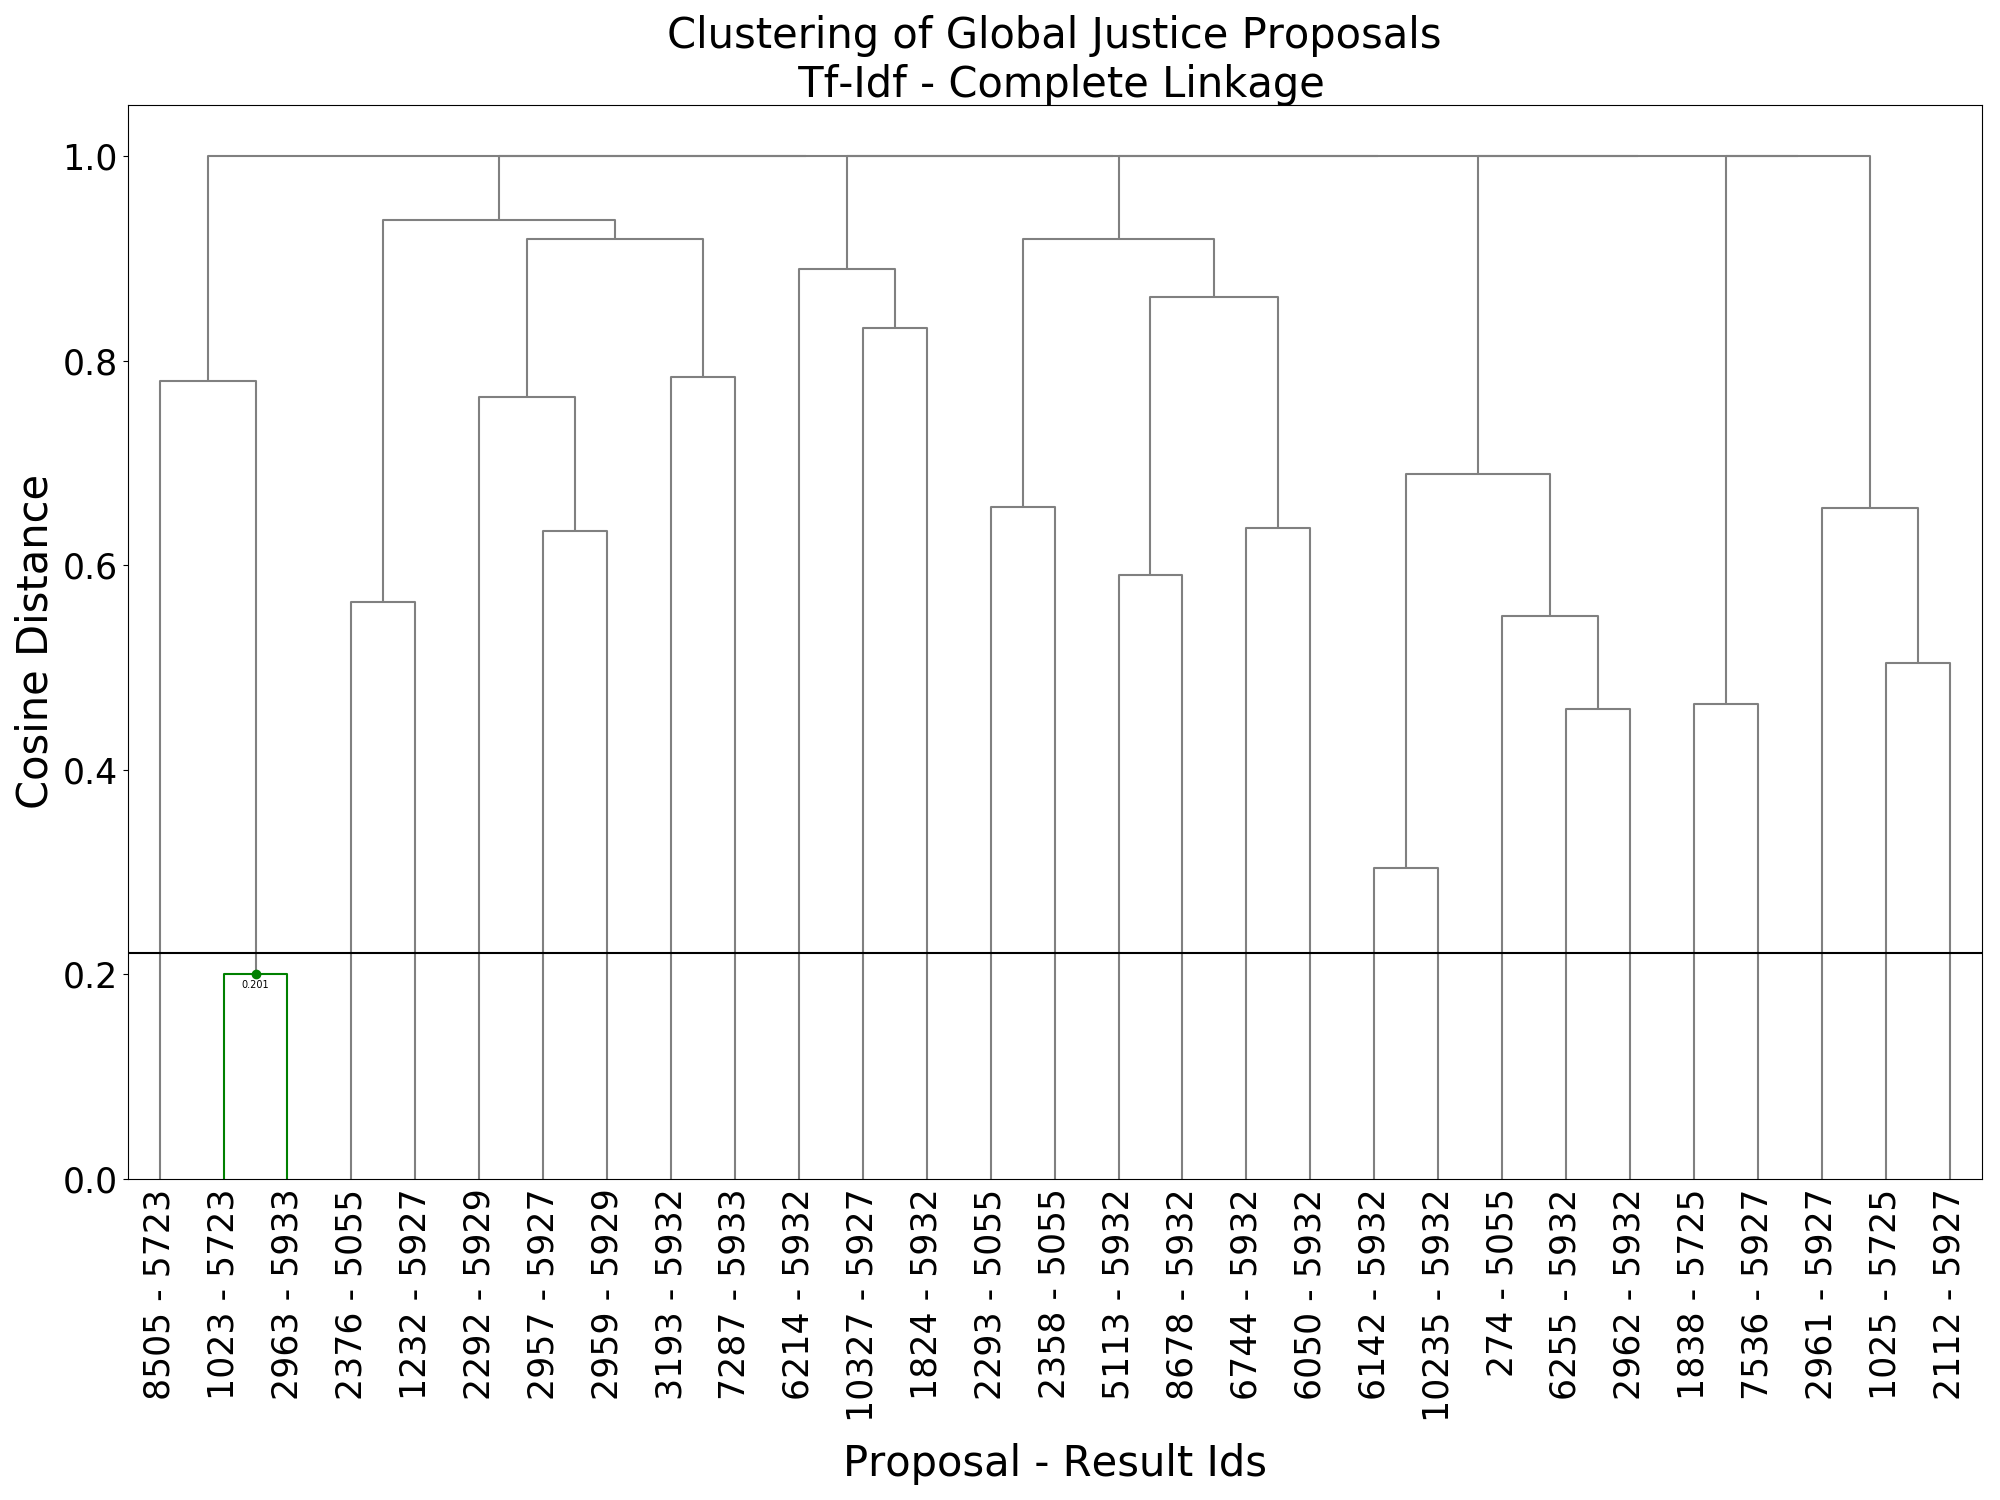
\includegraphics[width=\textwidth]{tfidf/BEST_PURITY_Global_Justice.png}
  \caption[]%
  {{\small Clustering with highest Purity.}}    
  \label{fig:gj.tfidf.purity}
  \end{subfigure}
  \vskip\baselineskip
  \begin{subfigure}[b]{0.48\textwidth}   
  \centering 
  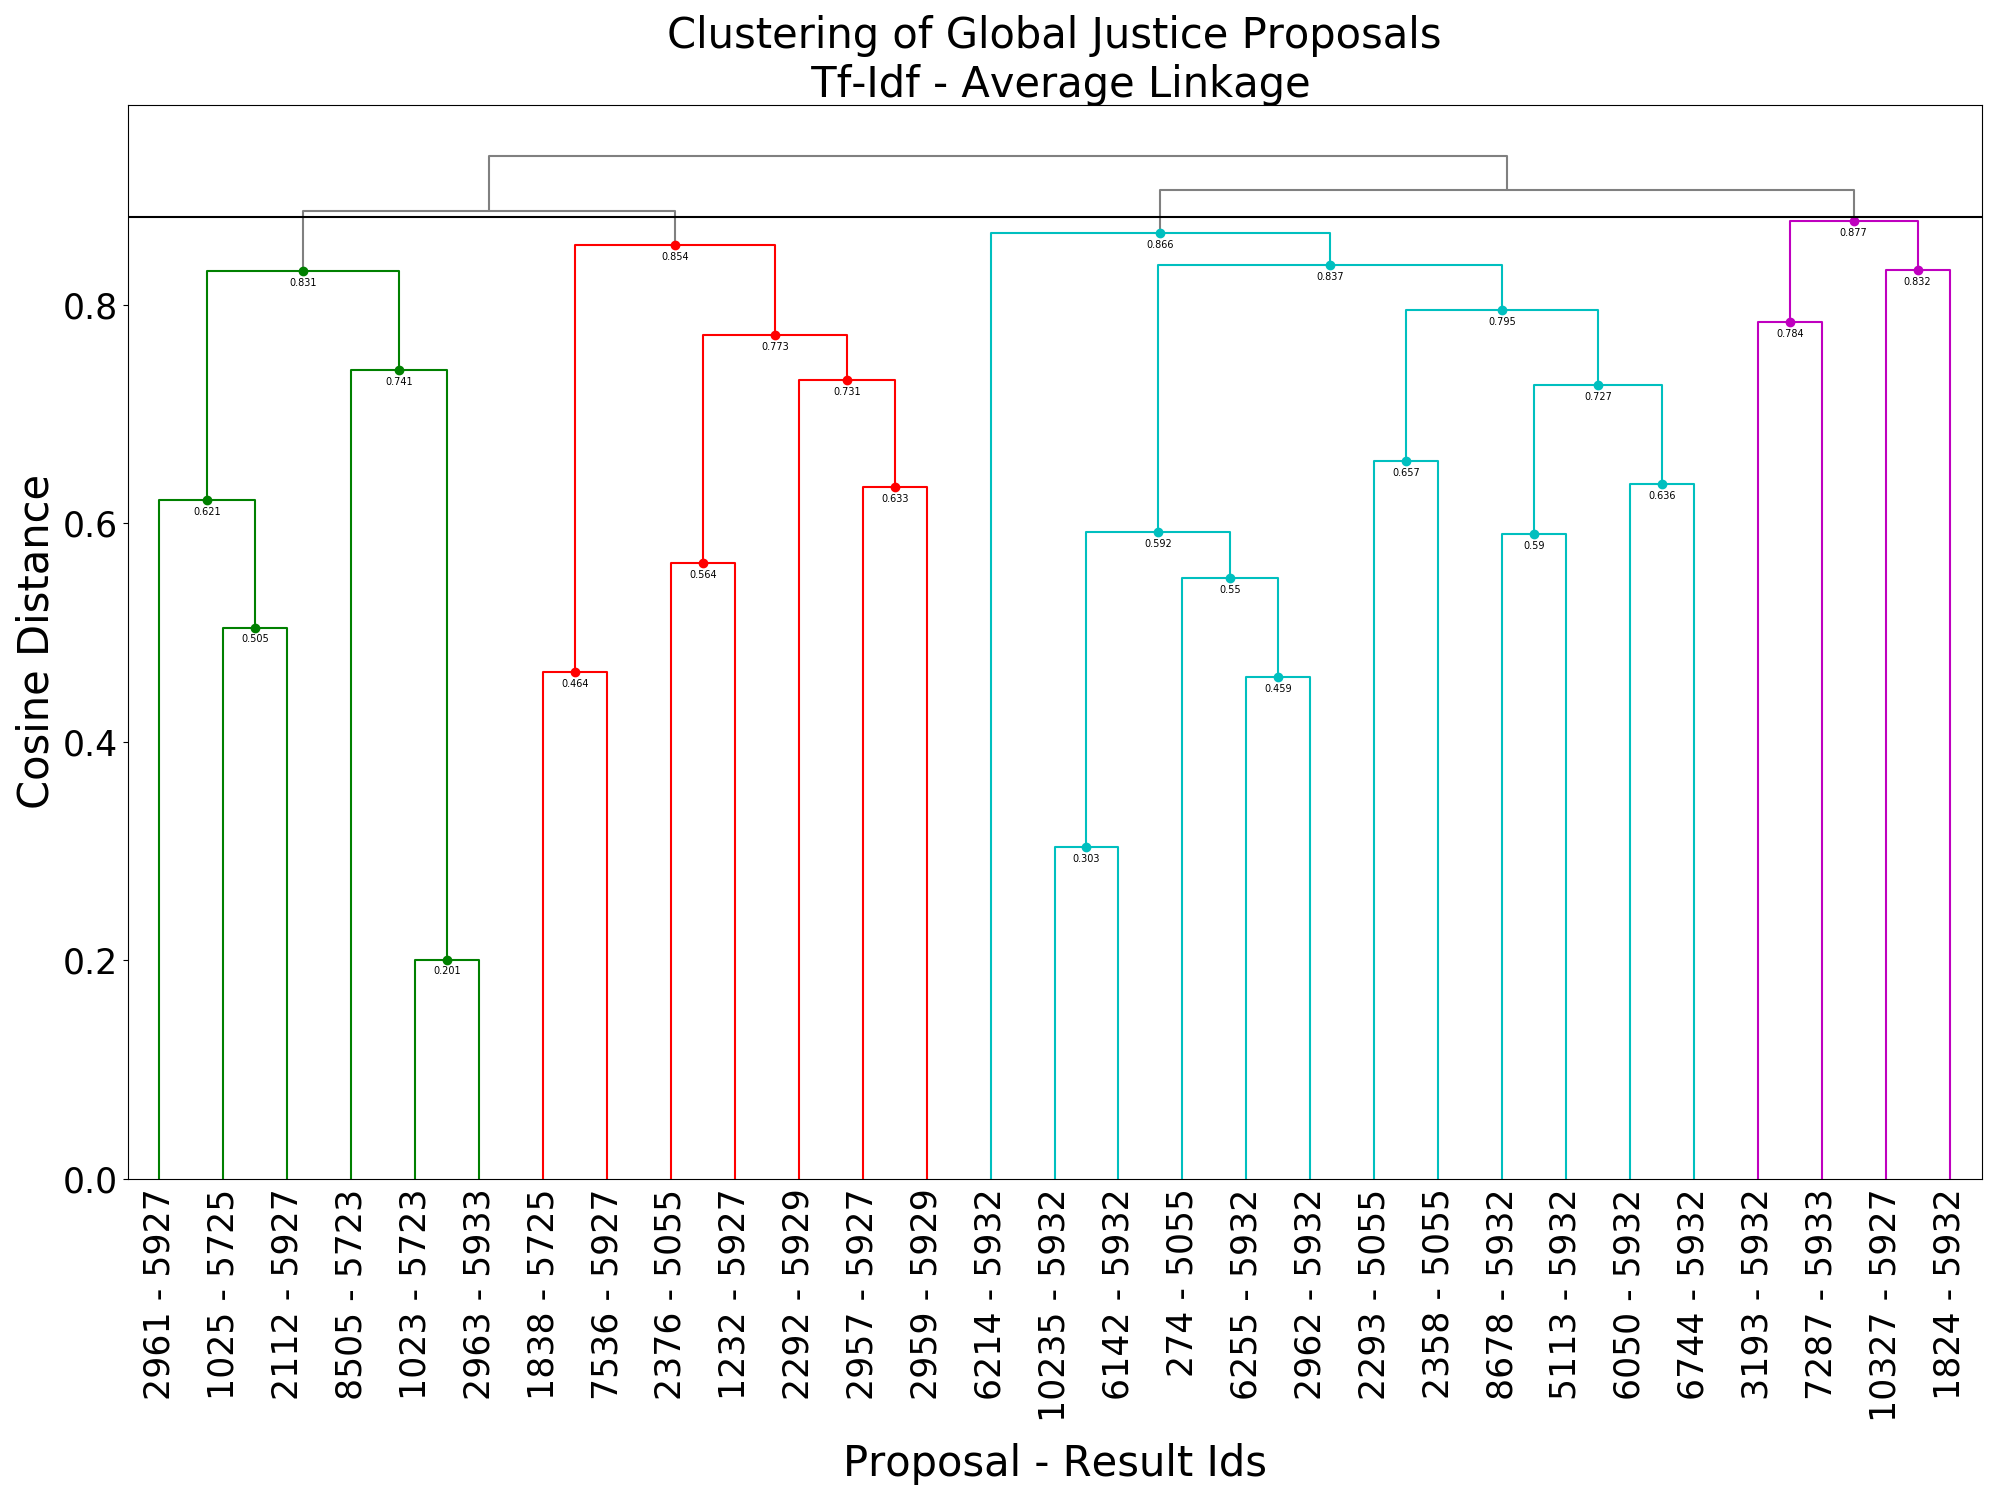
\includegraphics[width=\textwidth]{tfidf/BEST_ARI_Global_Justice.png}
  \caption[]%
  {{\small Clustering with highest ARI.}}    
  \label{fig:gj.tfidf.ari}
  \end{subfigure}
  \quad
  \begin{subfigure}[b]{0.48\textwidth}   
  \centering 
  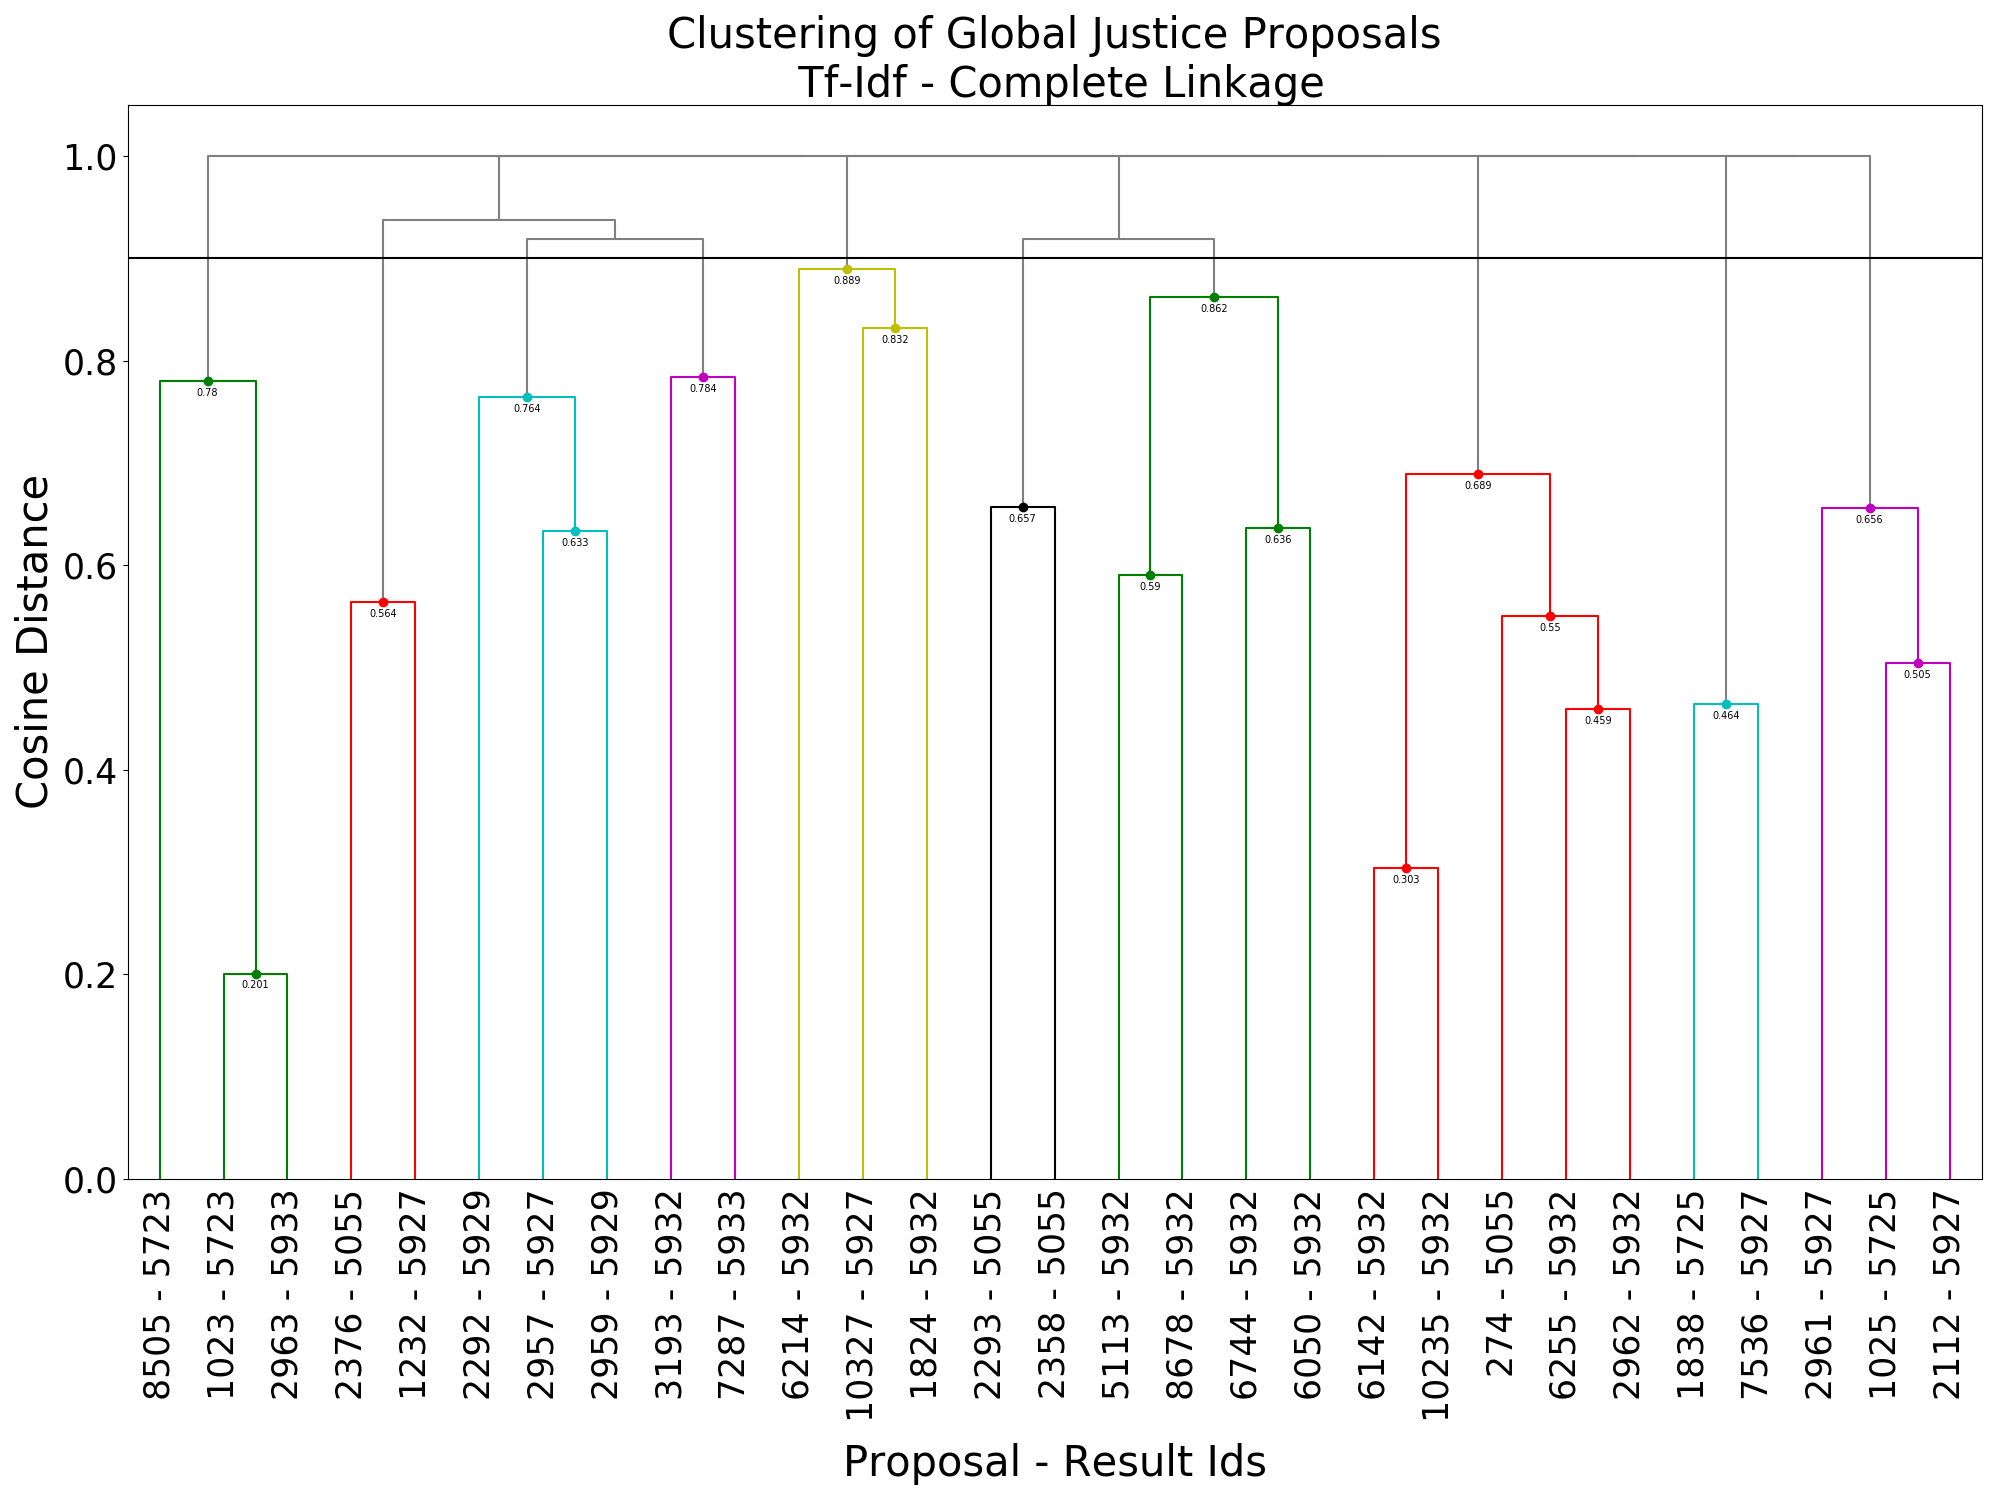
\includegraphics[width=\textwidth]{tfidf/BEST_SIL_Global_Justice.png}
  \caption[]%
  {{\small Clustering with highest Silhouette C.}}    
  \label{fig:gj.tfidf.sil}
  \end{subfigure}
\caption{Dendrogram with highest quality score of Global Justice Proposals for Tf-Idf.}
\label{fig:gj.tfidf.dendro}
\end{figure*}

% \begin{figure}[htpb]
% \centering
% 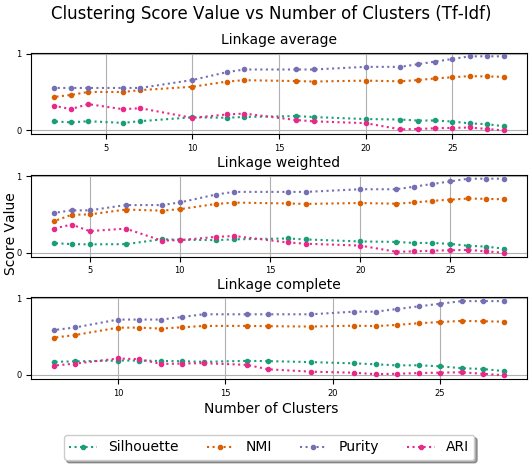
\includegraphics[width=10cm]{tfidf/clusters_score_tf-idf_Global_Justice.png}
% \caption{Global Justice Proposals quality metrics vs number of clusters (Tf-Idf).}
% \label{fig:gj.gj.tfidf.scores}
% \end{figure}
\FloatBarrier
\subsection{LSA Results}
In figure \ref{fig:gj.lsa.dendro} we can see the dendrograms for the best scores when using LSA. Dendrograms for the best NMI and purity have been ignored given the little information they provide. In these dendrograms we can see why LSA reached the highest silhouette coefficient in table (see table \ref{tab:negative.scores}) as this produce very well defined clusters with elements within the same cluster very close between them and far from elements in different clusters . LSA outputs very compact clusters, specially when compare to the output of Tf-Idf. The dimensionality reduction of the proposals' vectors removes noise from the output of Tf-Idf, which produces a sparse matrix.

\begin{figure*}[!htpb]
  \centering
  \begin{subfigure}[b]{0.48\textwidth}   
  \centering 
  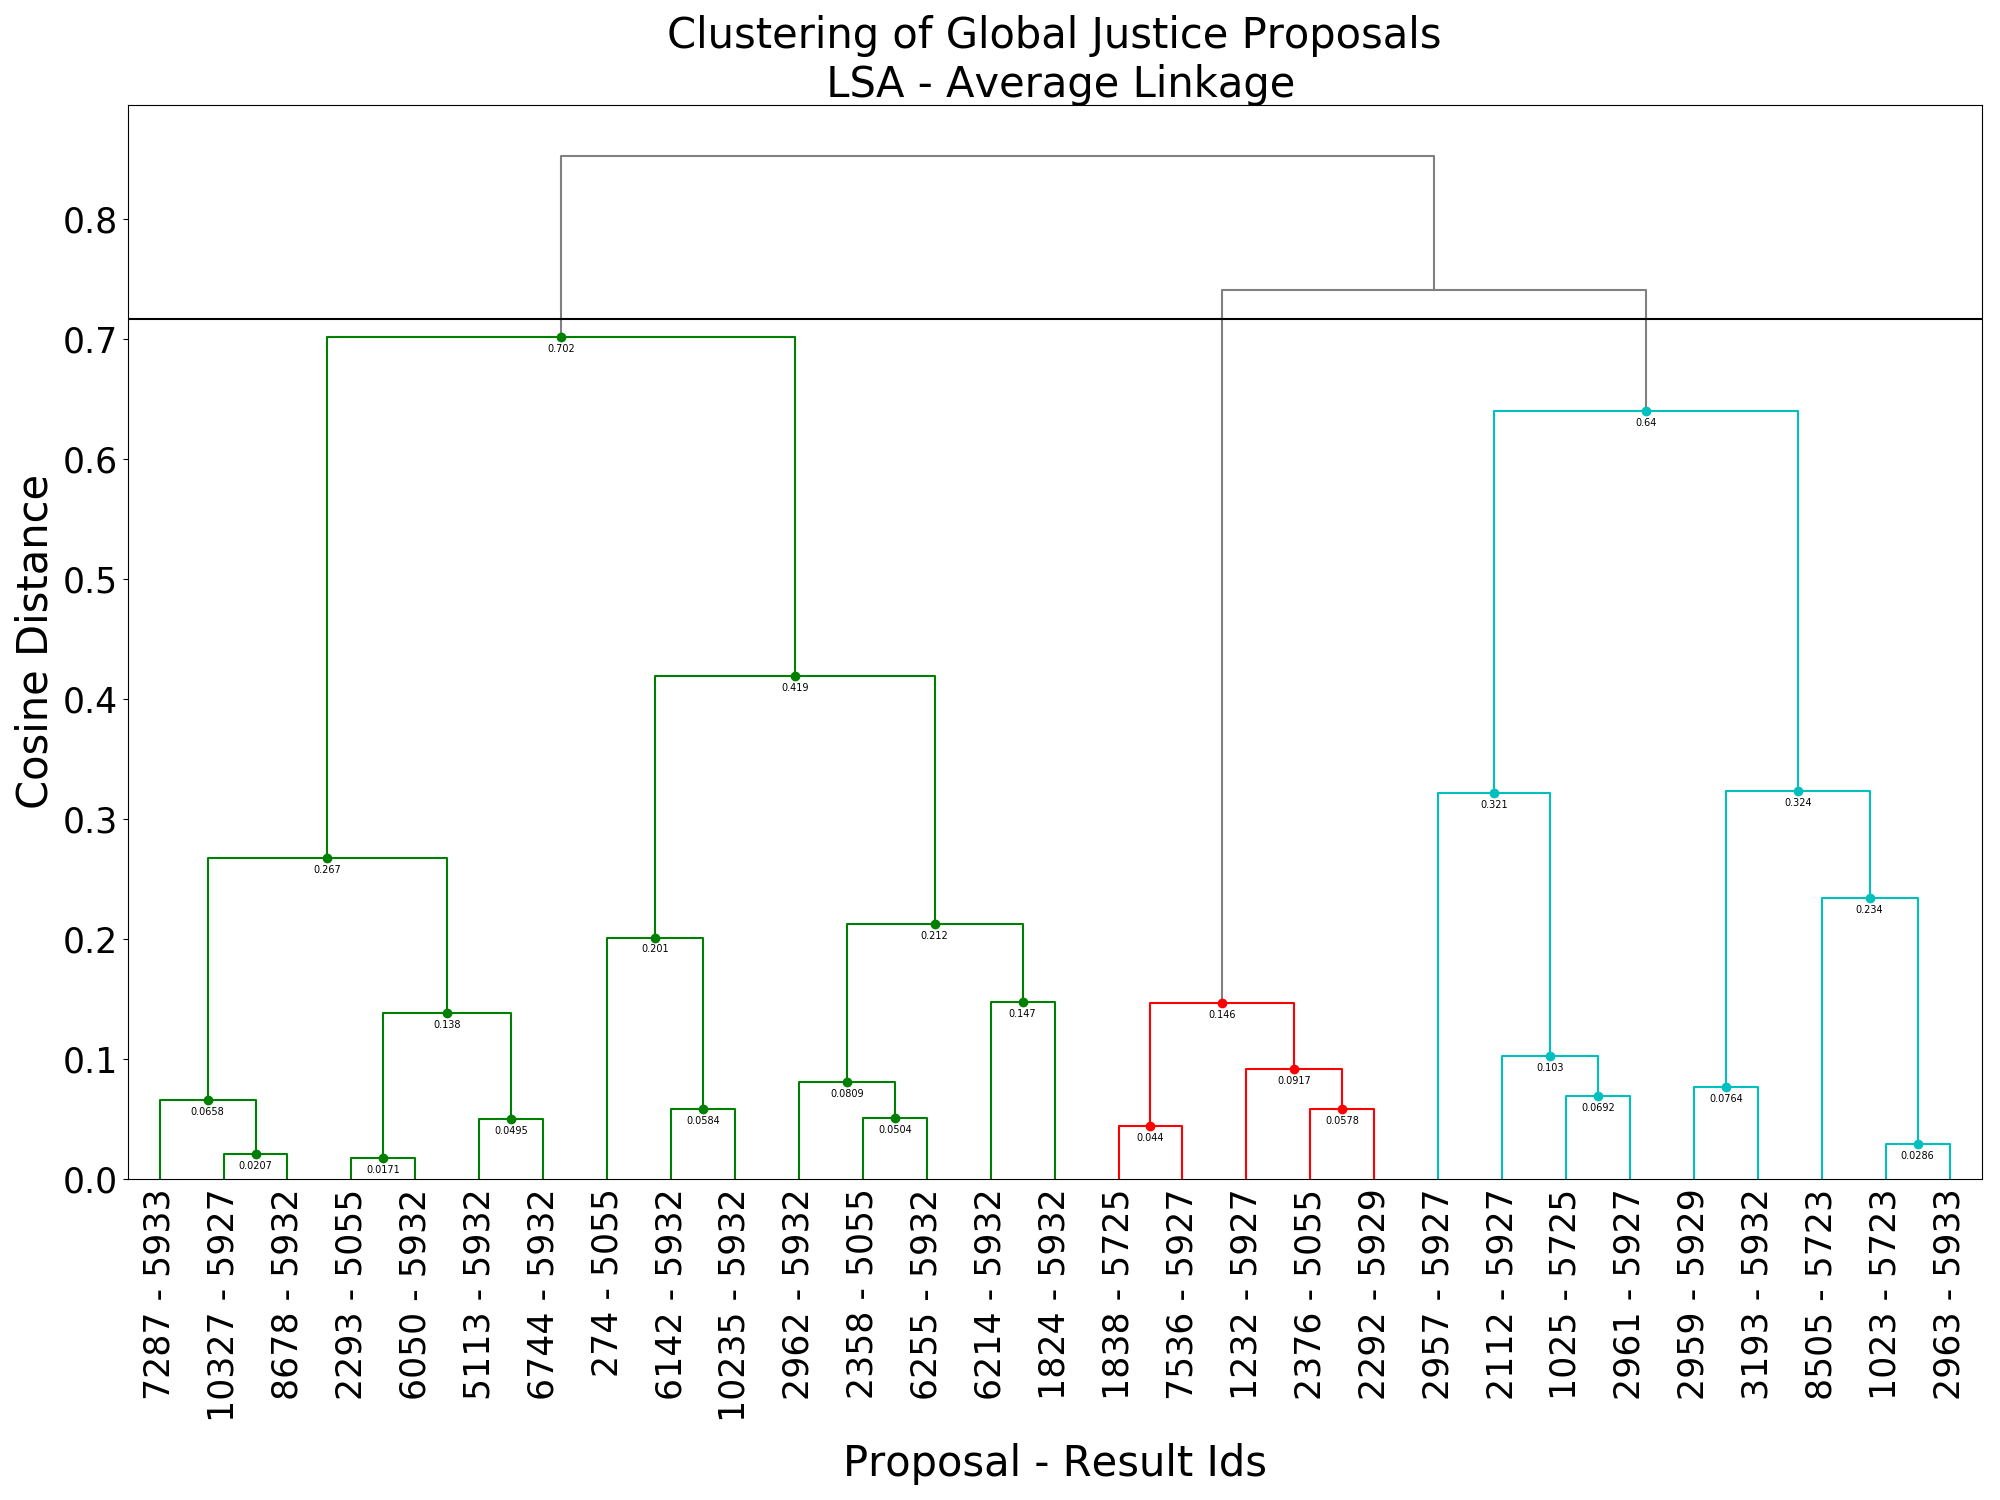
\includegraphics[width=\textwidth]{lsa/BEST_ARI_Global_Justice.png}
  \caption[]%
  {{\small Clustering with highest ARI.}}    
  \label{fig:gj.lsa.ari}
  \end{subfigure}
  \quad
  \begin{subfigure}[b]{0.48\textwidth}   
  \centering 
  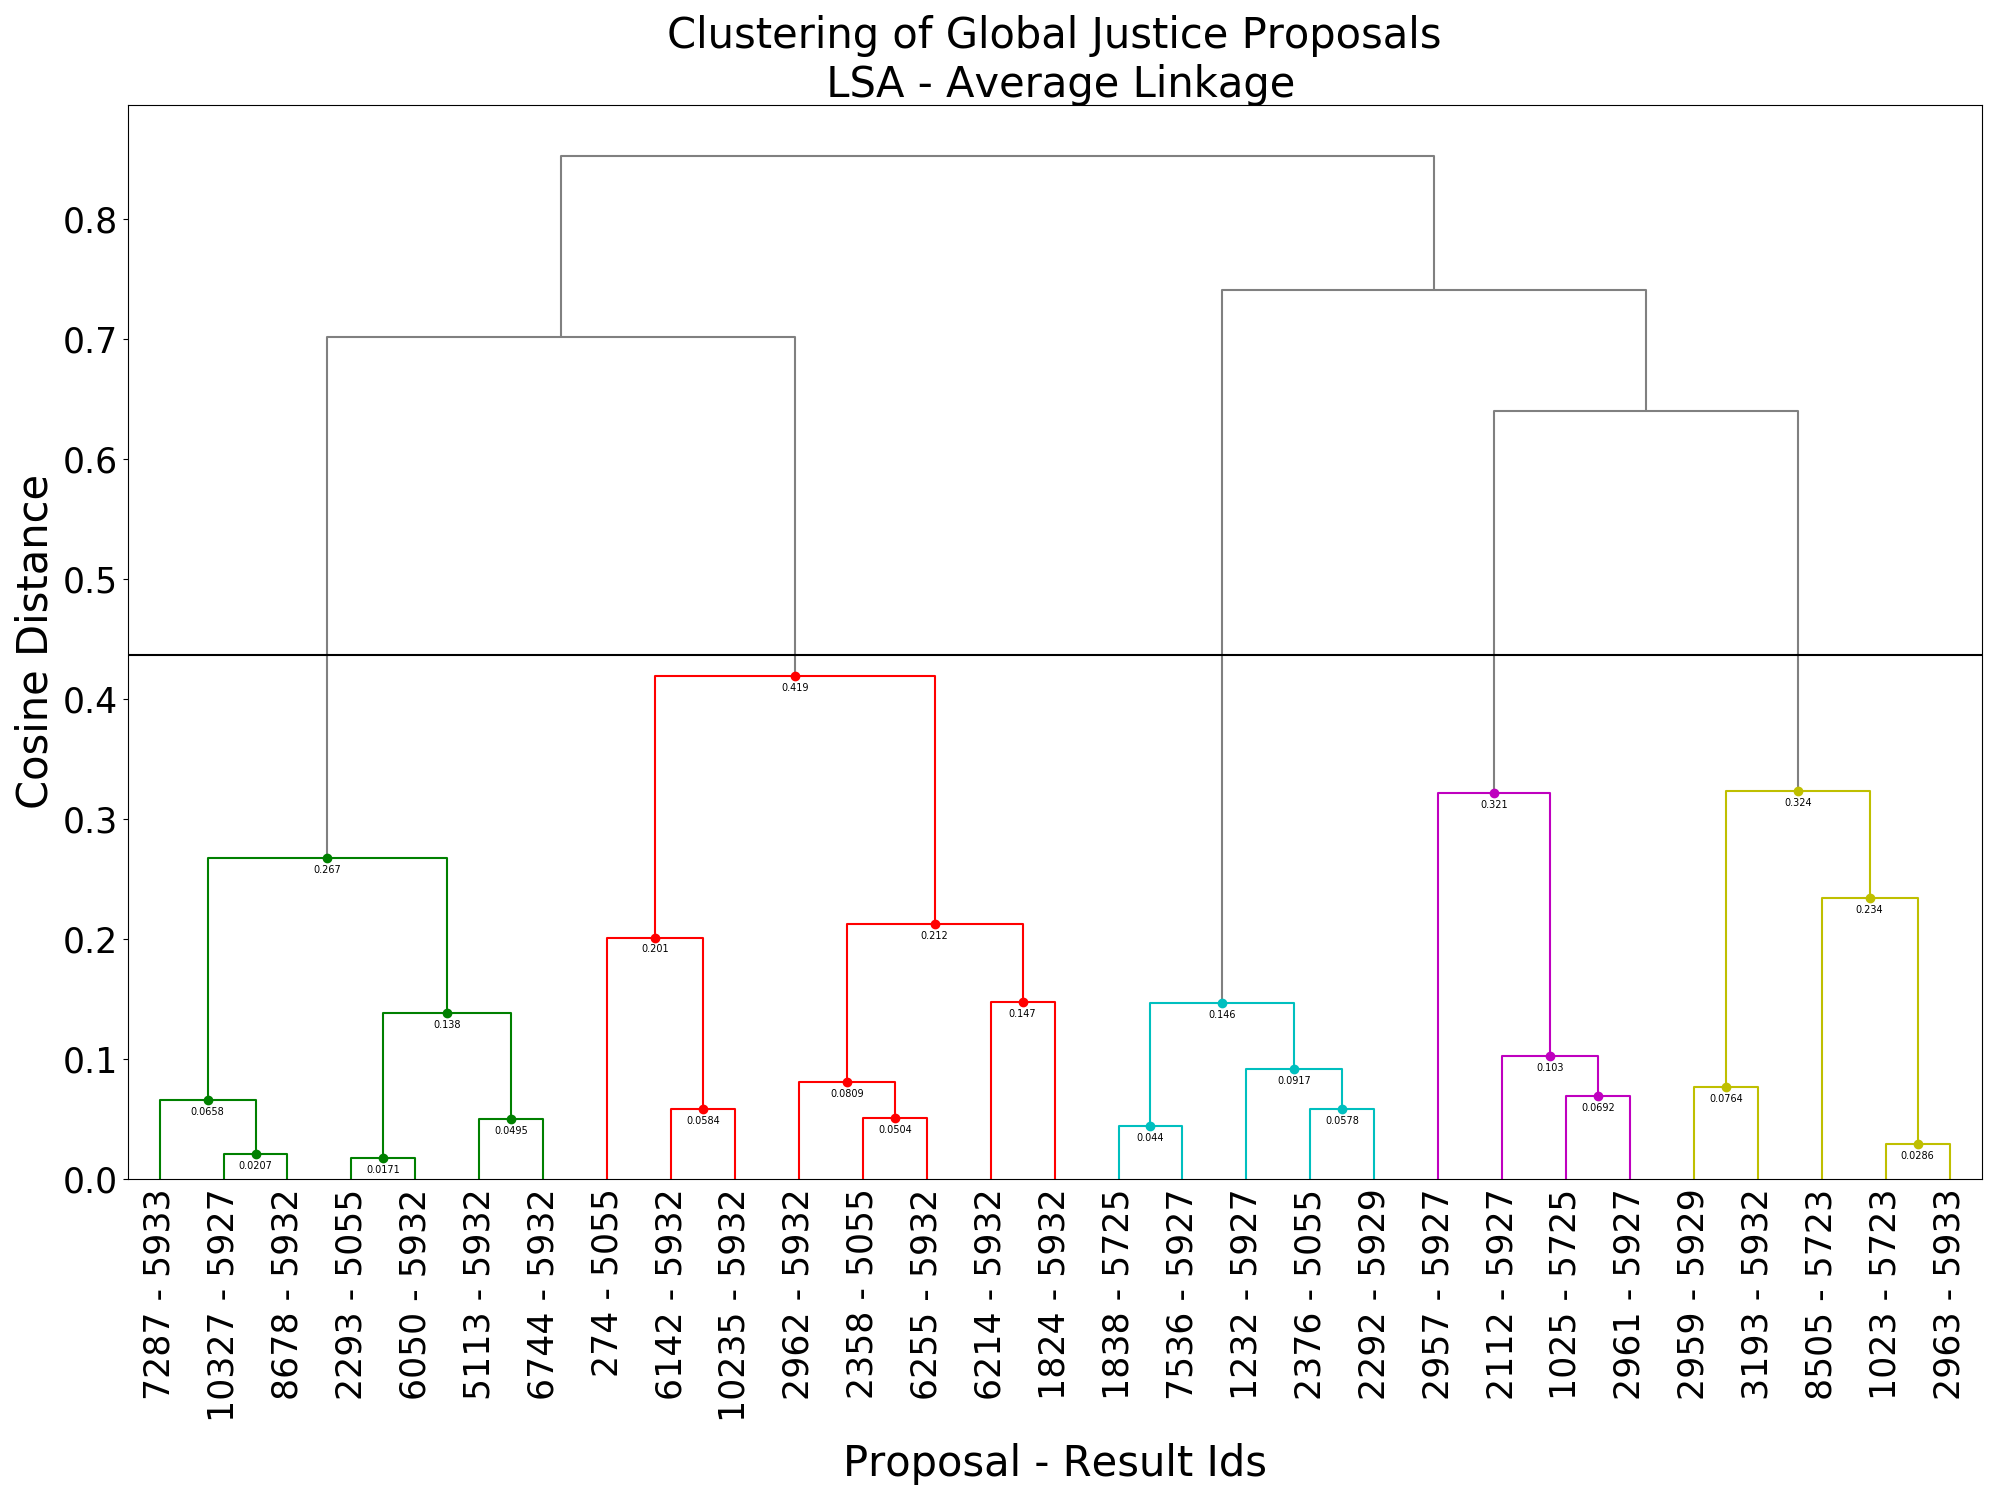
\includegraphics[width=\textwidth]{lsa/BEST_SIL_Global_Justice.png}
  \caption[]%
  {{\small Clustering with highest Silhouette C.}}    
  \label{fig:gj.lsa.sil}
  \end{subfigure}
\caption{Dendrogram with highest quality score of Global Justice Proposals for LSA.}
\label{fig:gj.lsa.dendro}
\end{figure*}

The highest ARI and Silhouette score was produced by the average linkage. Their differ in the cut height. In figure \ref{fig:gj.lsa.sil} five clusters were created which is the closest result to the actual number of clusters. From the clusters in \ref{fig:gj.lsa.sil} we can extract the following main topics per cluster:
\begin{enumerate}[itemsep=1pt,parsep=1pt]
\item Green cluster: Refugees.%Global justice, international network.
\item Red cluster: Refugees. 
\item Blue cluster: International cooperation, exchange of practices across cities.
\item Purple cluster: Global justice.
\item Yellow cluster: International network, human rights (the word Barcelona is present in all proposals of this cluster).
\end{enumerate}

When looking at the clusters in \ref{fig:gj.lsa.sil} we could see that the proposals in each cluster have a high degree of relation between them. If we split the dataset content into two main topics it would be very clear to define a group of proposals that speak about refugees and another group about international cooperations. This division would be perfectly recreated by LSA if we cut the dendrogram at 0.8.

% \begin{figure}[htpb]
% \centering
% 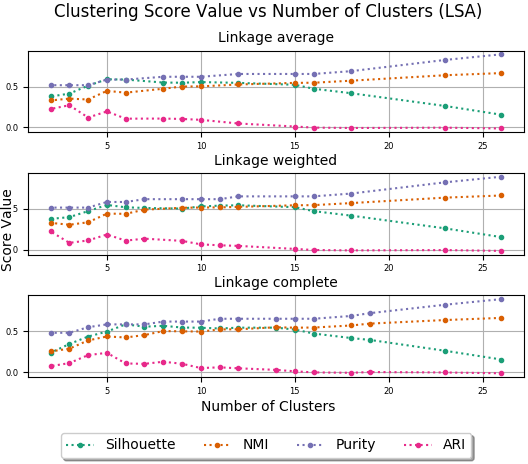
\includegraphics[width=10cm]{lsa/clusters_score_lsa_Global_Justice.png}
% \caption{Global Justice Proposals quality metrics vs number of clusters (LSA).}
% \label{fig:gj.lsa.scores}
% \end{figure}
\FloatBarrier
\subsection{Word2Vec Results}
In figure \ref{fig:gj.word2vec.dendro} we can see the resulting dendrogram from Word2Vec + Average linkage. In this case the silhouette coefficient is maximized when only two clusters are defined (see figure \ref{fig:gj.word2vec.sil}). It can be noticed that silhouette coefficient tends to cut the dendrogram at the point where the highest inter clustering distance is found. 

Looking at figure \ref{fig:gj.word2vec.ari} three clusters were defined:
\begin{enumerate}[itemsep=1pt,parsep=1pt]
\item Green cluster: International cooperation, exchange of practices across cities, refugees.
\item Red cluster: Global justice, refugee.
\item Blue cluster: International cooperation, human rights, global justice.
\end{enumerate}
We can see that Word2Vec failed to split proposals into groups of related topics. This result was unexpected, given that since its publication in 2013 many researches have used Word2Vec to improve state-of-the-art algorithms in fields like natural language \cite{semantic.short}. Certainly, there is a lack of investigation on how effective is Word2Vec capturing the semantical meaning from short sentences \cite{semantic.short}.
\begin{figure*}[!htpb]
  \centering
  \begin{subfigure}[b]{0.60\textwidth}   
  \centering 
  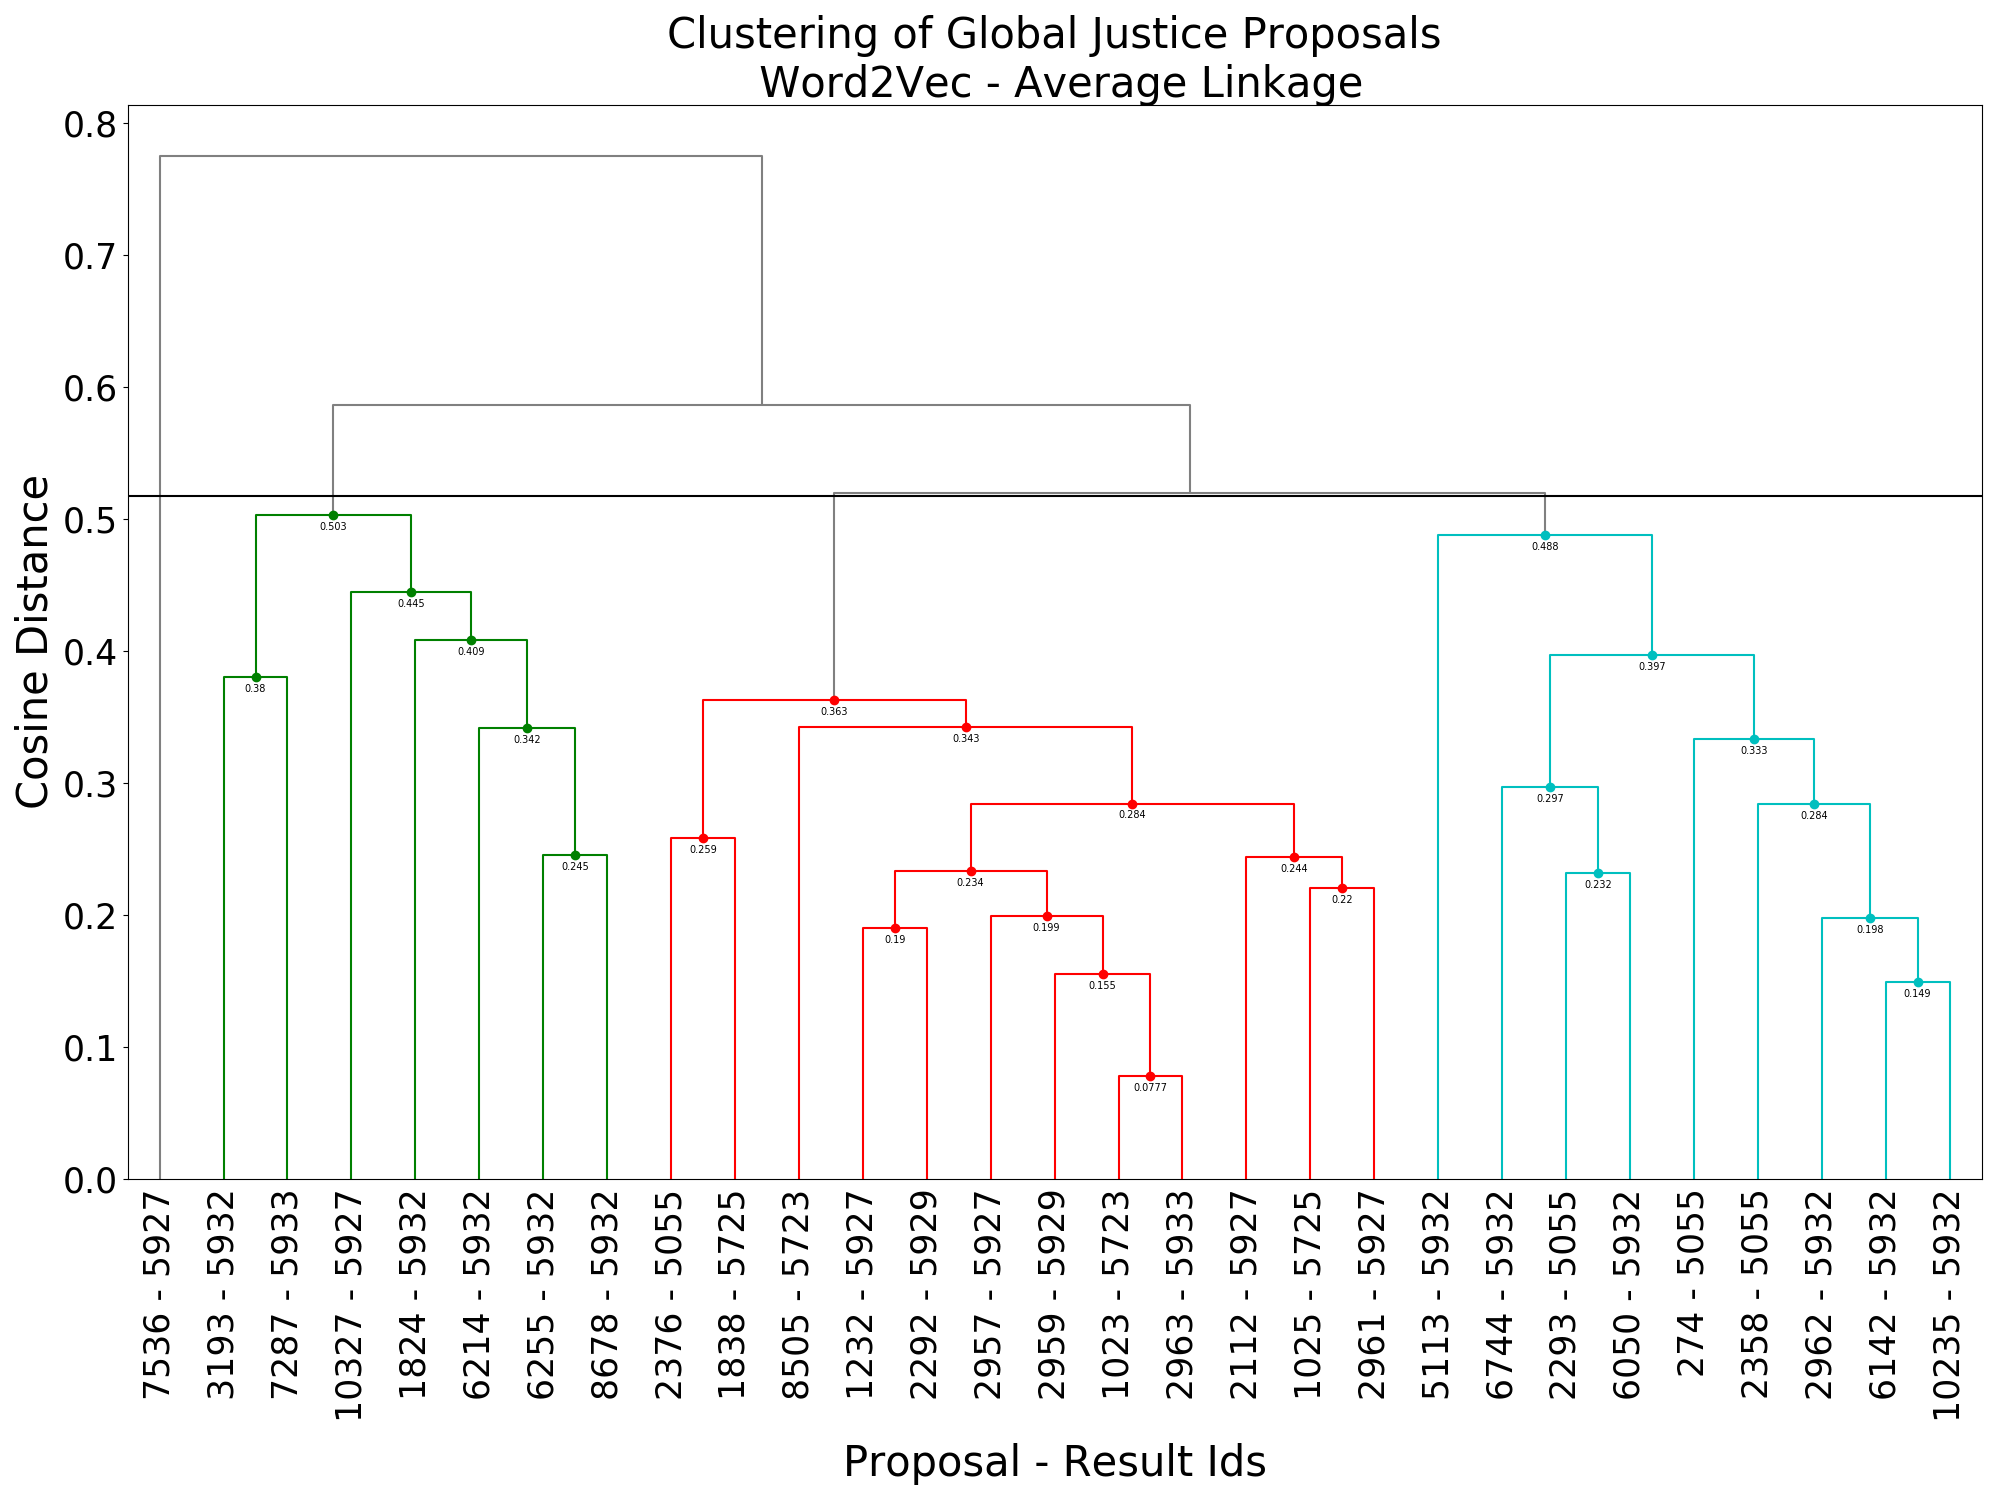
\includegraphics[width=\textwidth]{word2vec/BEST_ARI_Global_Justice.png}
  \caption[]%
  {{\small Clustering with highest ARI.}}    
  \label{fig:gj.word2vec.ari}
  \end{subfigure}
  \quad
  \begin{subfigure}[b]{0.60\textwidth}   
  \centering 
  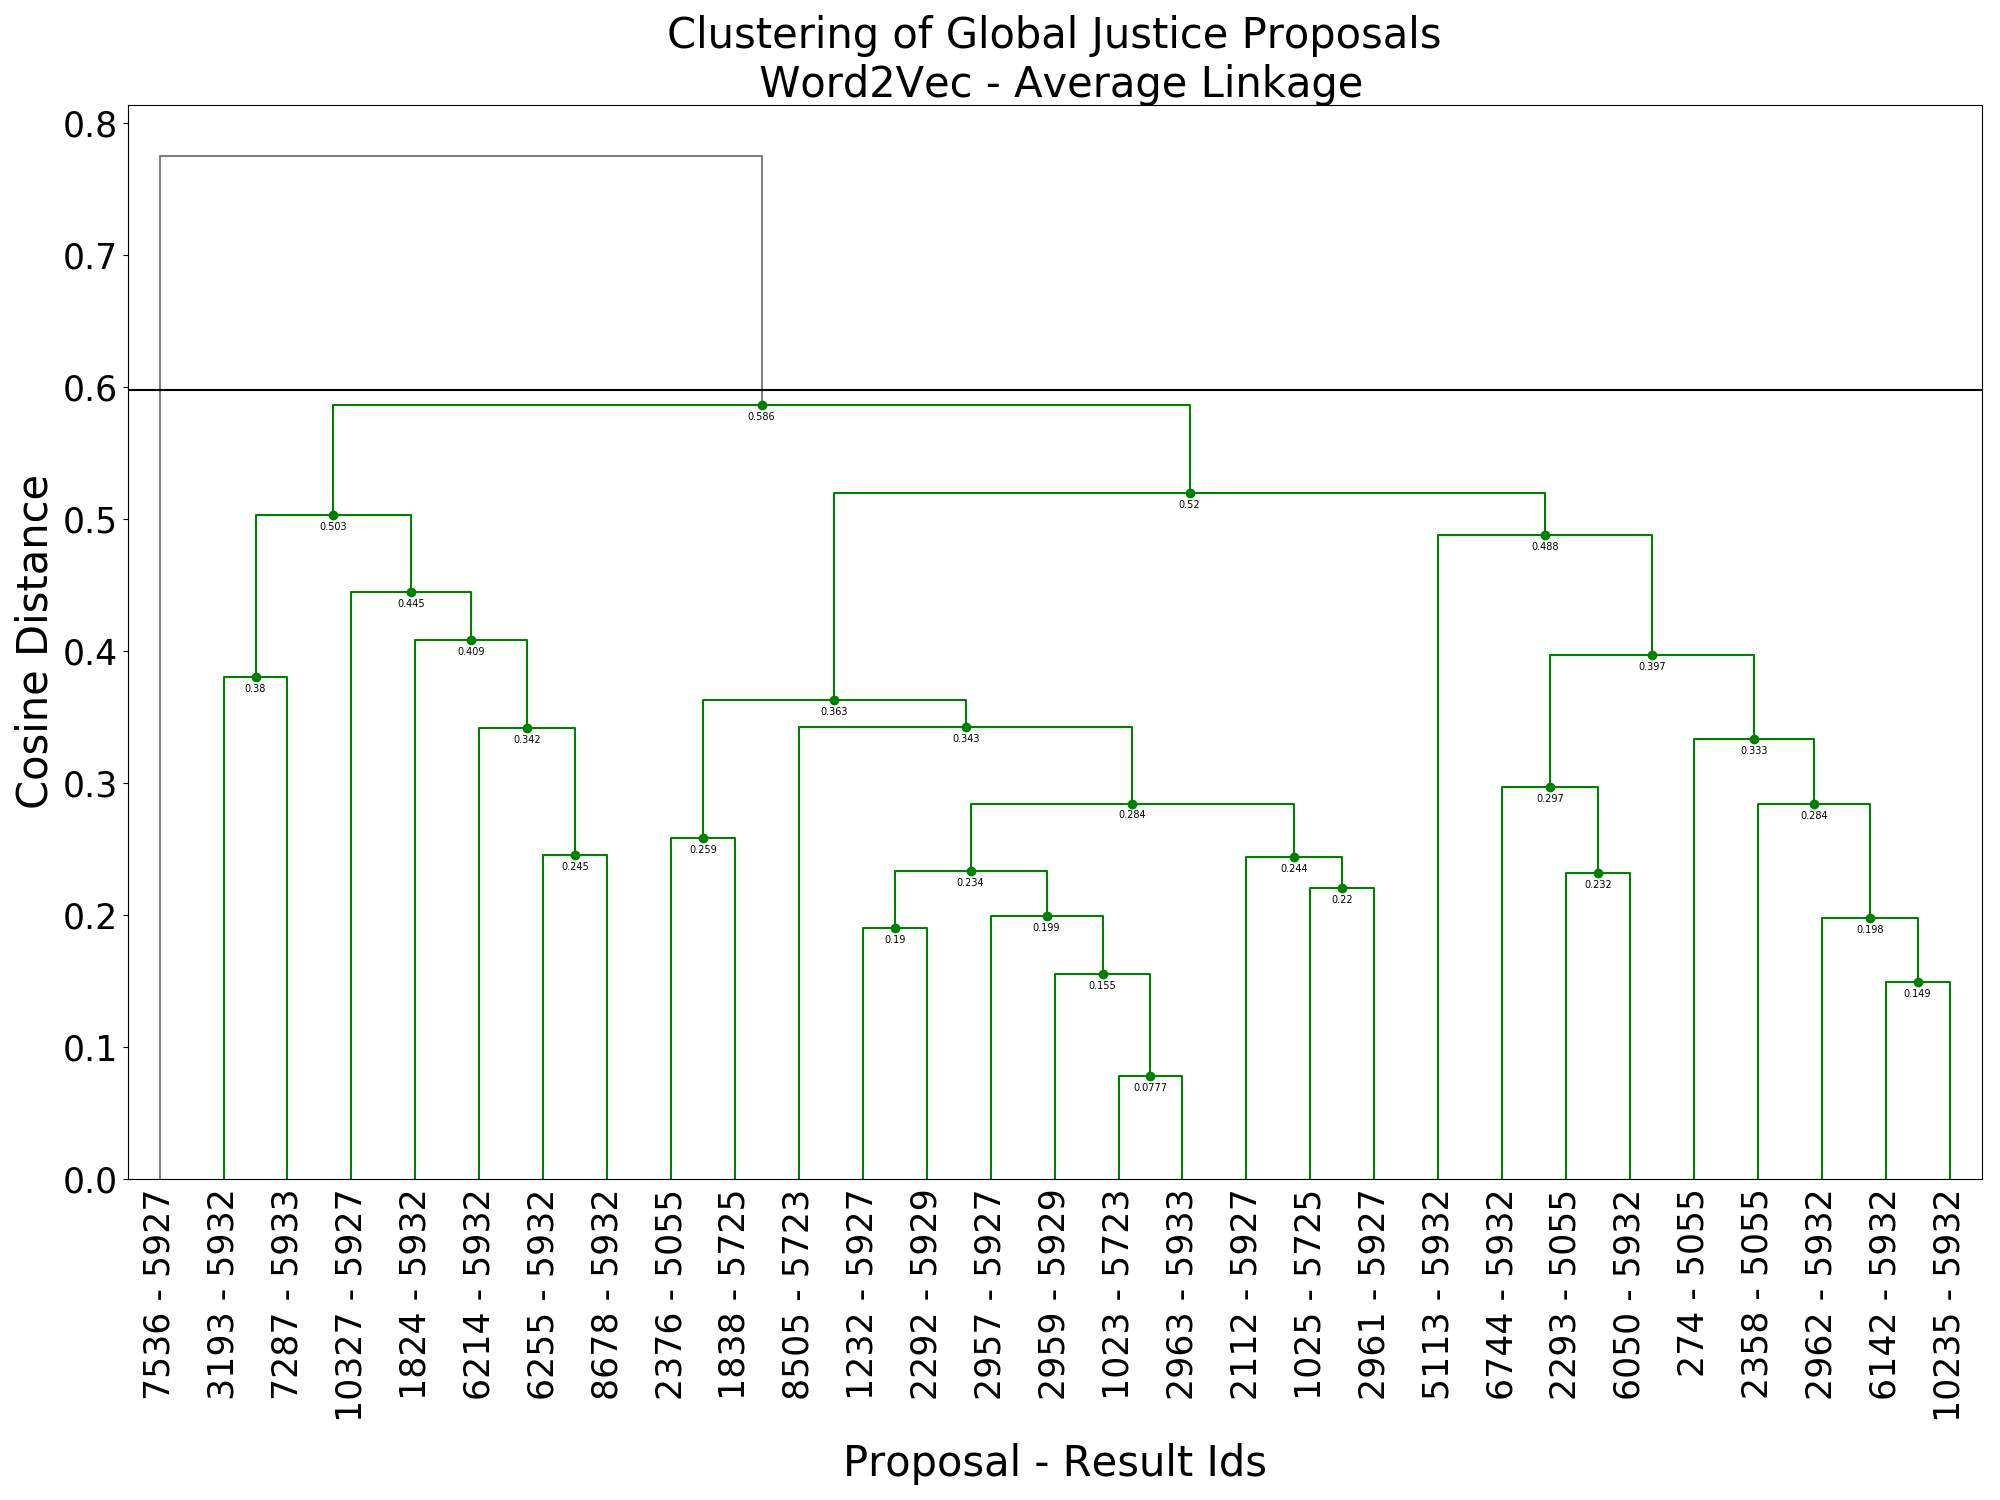
\includegraphics[width=\textwidth]{word2vec/BEST_SIL_Global_Justice.png}
  \caption[]%
  {{\small Clustering with highest Silhouette C.}}    
  \label{fig:gj.word2vec.sil}
  \end{subfigure}
\caption{Dendrogram with highest quality score of Global Justice Proposals for Word2Vec.}
\label{fig:gj.word2vec.dendro}
\end{figure*}
    

% \begin{figure}[!htpb]
% \centering
% 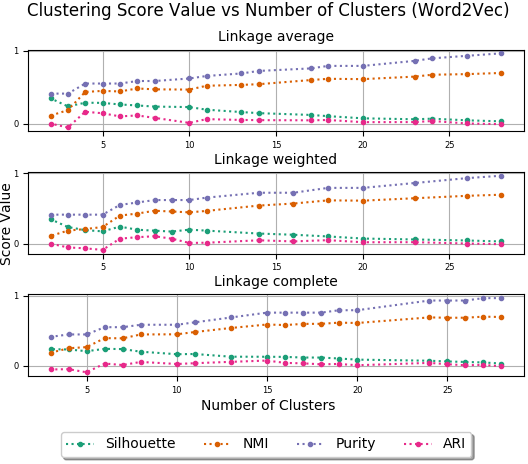
\includegraphics[width=10cm]{word2vec/clusters_score_word2vec_Global_Justice.png}
% \caption{Global Justice Proposals quality metrics vs number of clusters (Word2Vec).}
% \label{fig:gj.word2vec.scores}
% \end{figure}
\FloatBarrier

\scriptsize 
\begin{spacing}{1}
\begin{longtable}{m{30mm}|m{90mm}|c @{\hskip 1mm} c}
\hline
Title & Description & Proposal & Result\\
\hline
\hline
\endhead
 Actions on cooperation. & Promote shared projects with other reference cities to: share experience, visibilize the world that it is possible to do it in a different way with example around the world. & 2376 & 5055, 5927 \\ \hline
 Start the "Refuge" plan & The District of the Eixample undertakes to develop the "Refuge" plan and to promote the involvement of entities and groups in the different neighborhoods in this plan. & 274 & 5055  \\ \hline
 Initiatives with refugees. & creation of shelters, reception. & 2293 & 5055, 5932  \\ \hline
 Attention to refugees. & Barcelona City Refuge, neighborhood committed to the refugees, platform creation or support group & 2358 & 5055, 5932  \\ \hline
 Participate in international networks to support the rights of migrants & It strives to coordinate and to be part of the international initiatives in defense of the rights of the migrants, as much at institutional level as citizen. & 8505 & 5723  \\ \hline
 Commit Barcelona to the global fight for human rights & Increase efforts to make public debate, support organizations that work for regional justice and initiate processes of international impact to contribute to the achievement of a system of global governance that protects the human rights of people and peoples in the Euro-Mediterranean region. & 1023 & 5723  \\ \hline
 Educate for global justice & Progressively increase the weight of education for global justice.We must move towards an identified citizenry with a solidarity Barcelona and committed to global justice, and involved in the different transnational networks that work in this regard from civil society. & 1025 & 5725  \\ \hline
 Report international cooperation projects & disseminate good practices, horizontally and vertically, to share and improve the actions that are carried out & 1838 & 5725  \\ \hline
 Insubmission to TTP, TTIP and TISA. & Declare Barcelona as a city insubmised in the treaties of the TTP, TTIP and TISA, to make a campaign for information and dissemination for the commerce of the proximity of this treaty and its involvement in trade. & 10327 & 5927 \\ \hline
 Renew the spaces and processes of participation and sensitization of the city's agents in matters of global justice & Taking into account the changes suffered during the last years in the set of actors related to global justice, it is advisable to review and search the most effective ways of co-participation between citizens, the sector, public institutions and the City Council. & 2961 & 5927 \\ \hline
 Exchange of good practices between European cities & Export and import activities and good practices that are working & 7536 & 5927 \\ \hline
 Develop a global action plan and justice 2016-2020 & The outer action plan will outline the guidelines of the city's foreign policy in all its dimensions (governance, relations with other international cities, international networks, economic relations, culture, cooperation, etc.).It is an instrument of definition and planning of the public policy of global justice, which is especially vigilant for the coherence of the external action of the municipal Government. & 2957 & 5927 \\ \hline
 Reinforce the policies of relations and international cooperation of the city council & Strengthen the relationship and cooperation of the city council with other cities around the world and its external projection in order to learn from the best practices and promote the development and inclusion experiences driven locally.Work in horizontal networks of cities and deepen development cooperation projects. & 1232 & 5927 \\ \hline
 Transition towards a model of cooperation aimed at global justice & Work on sensitization and solidarity actions. & 2112 & 5927 \\ \hline
 Measures on cooperation. & Promote a municipal cooperation network to act and move forward with the major issues that concern the State and Europe: the economic model, distribution of wealth, consumer culture, ecology, etc. & 2292 & 5929 \\ \hline
 Coordinate and strengthen the international networks present in the city & Develop a work strategy that strengthens the principles and values ​​that define the municipal cooperation, based on the fact that in Barcelona there are headquarters and general secretariats of the main international municipal networks, and it is the city that participates in a greater number of international networks, both generalist and thematic (in key areas such as the environment, the fight against climate change, local governance, education, etc.).Guarantee also that this know how to make use of the economic fabric of the city. & 2959 & 5929 \\ \hline
 Increase support for all refugees & Mitjans school plan, family plan ... & 6142 & 5932 \\ \hline
 Incorporate LGBT perspective in the refugee support plan & Incorporate the LGTBI perspective in the refugee support plan and take into account its rights as LGBT people. & 10235 & 5932 \\ \hline
 Motion for refugee reception & Join the motion approved by the District Council of the District of Sants-Montjuic by the Senate Sectoral Council. & 5113 & 5932  \\ \hline
 Create reception spaces for immigrant and refugee population & Often the population that arrives in Barcelona fleeing poverty or conflicts in their countries is relocated.You need to create reception and education spaces where you can meet your first needs. & 6744 & 5932 \\ \hline
 Help Syrian people & Barcelona should give an example and collaborate with economic funds with pro-active open arms every day where its volunteers play their lives saving people who flee from the war in Syria.It is unfortunate as a cosmopolitan and open city Enacara has not acted in this great humanitarian crisis with concrete facts and easy to carry out & 3193 & 5932\\ \hline
 Barcelona city refuge in Sarrià - Sant Gervasi & Support the proposal "start the Barcelona city refugee plan" and let it be set up in this district. & 6255 & 5932 \\ \hline
 Start the plan "Barcelona, ​​a city refuge" & Start up an operational and strategic plan for the reception of the city.To create a stable and permanent support structure for refugees and asylums that is complementary to state programs, with their own criteria and in collaboration with entities that work on the subject.Pay special attention to asylum seekers who are left out of the state social support program.Create a city-to-city cooperation plan for the high-density municipalities receiving refugees and migrants. & 2962 & 5932 \\ \hline
 Withdrawal of the EU flag to any official entity in Barcelona & Withdrawal of the EU flag to any official entity of Barcelona as a sign of rejection for the lamentable action that is being carried out with the refugees & 6214 & 5932 \\ \hline
 Leadership of Barcelona host city. & The city of Barcelona, ​​with the city council at the head, leads the reception of refugees. & 8678 & 5932 \\ \hline
 Create a bank of resources for refugees at the level of the District connected to the Generalitat in two levels (reception and awareness) & The reception of refugees in the city must be planned, work in conjunction with the Generalitat and establish measures to: - The reception (accommodation, support, language, etc.) - Awareness (educational centers and citizenship in general) & 6050 & 5932 \\ \hline
 Participation in the Social Area Barcelona City Refuge & Participation in the Social Area Barcelona City Refuge & 1824 & 5932 \\ \hline
 Engage in the reconstruction of the city of Kobane, in the Kurdish region of Syria. & The city of Kobane was a battle scene of the Kurdish militia against Daesh (Islamic state).The battle was won but the city was destroyed by 70\%.Now you have to rebuild it.Thus emancipating policies in the Middle East are supported and conditions are created so that the population can return instead of fleeing to Europe. & 7287 & 5933 \\ \hline
 Boost Barcelona as the capital for peace in the Mediterranean & Promote cooperation agreements and transnational twinning with cities considered as the arrival points of refugees and migrants from the Mediterranean in coordination with existing networks and the Refugee Cities Network.Increase the efforts to make a public debate, support organizations that work for regional justice and initiate processes of international impact to contribute to the achievement of a global governance system that protects the human rights of people and the towns in the region. & 2963 & 5933 \\ \hline
\caption{Global Justice proposals.}
\label{tab:negatives} \\
\end{longtable}
\end{spacing}
\normalsize
\newpage
